\documentclass[12pt]{article}

% ---- Packages ----
\usepackage[T1]{fontenc}
\usepackage{lmodern}
\usepackage{amsmath, amssymb, amsthm}
\usepackage{booktabs}
\usepackage{graphicx}
\usepackage[authoryear, round]{natbib}
\usepackage{hyperref}
\usepackage[margin=1in]{geometry}
\usepackage{setspace}
\usepackage{enumitem}
\usepackage{caption}
\usepackage{array}
\usepackage{multirow}
\usepackage{xcolor}
\usepackage{float}

% ---- Theorem environments ----
\theoremstyle{plain}
\newtheorem{theorem}{Theorem}
\newtheorem{proposition}[theorem]{Proposition}
\newtheorem{lemma}[theorem]{Lemma}
\newtheorem{corollary}[theorem]{Corollary}
\theoremstyle{definition}
\newtheorem{definition}[theorem]{Definition}
\newtheorem{axiom}{Property}
\theoremstyle{remark}
\newtheorem{remark}[theorem]{Remark}
\newtheorem{example}[theorem]{Example}
\newtheorem{conjecture}[theorem]{Conjecture}

% ---- Formatting ----
\onehalfspacing
\hypersetup{colorlinks=true, linkcolor=blue, citecolor=blue, urlcolor=blue}

% ---- Custom commands ----
\newcommand{\R}{\mathbb{R}}
\newcommand{\N}{\mathbb{N}}
\newcommand{\bfy}{\mathbf{y}}
\newcommand{\bfz}{\mathbf{z}}
\newcommand{\bfone}{\mathbf{1}}
\newcommand{\D}{\mathcal{D}}

% Generated by code/pip_disagreement.py -- do not edit by hand.
\newcommand{\PipPairs}{1{,}955}
\newcommand{\PipCountries}{143}
\newcommand{\PipYearMin}{1963}
\newcommand{\PipYearMax}{2025}
\newcommand{\PipDistributions}{2{,}588}
\newcommand{\PipDistCountries}{172}
\newcommand{\PipGiniMaxDiff}{0.0039}
\newcommand{\PipMldMaxDiff}{0.017}
\newcommand{\PipShareDom}{38\%}
\newcommand{\PipNDom}{738}
\newcommand{\PipShareCross}{62\%}
\newcommand{\PipShareSingle}{38\%}
\newcommand{\PipShareCrossDecile}{36\%}
\newcommand{\PipShareCrossTieOne}{29\%}
\newcommand{\PipShareCrossTieTwo}{16\%}
\newcommand{\PipTpAgreeCrossTieOne}{27\%}
\newcommand{\PipTpAgreeCrossTieTwo}{20\%}
\newcommand{\PipShareMulti}{24\%}
\newcommand{\PipTpAgreeAll}{70\%}
\newcommand{\PipTpAgreeCross}{51\%}
\newcommand{\PipTpDisMaterial}{9\%}
\newcommand{\PipNMaterial}{754}
\newcommand{\PipDtsAgreeCross}{65\%}
\newcommand{\PipTpDisMaterialCross}{23\%}
\newcommand{\PipNMaterialCross}{296}
\newcommand{\PipTpAgreeBigCross}{87\%}
\newcommand{\PipNBigCross}{580}
\newcommand{\PipNMicroPairs}{1{,}874}
\newcommand{\PipShareCrossMicro}{63\%}
\newcommand{\PipTpAgreeCrossMicro}{51\%}
\newcommand{\PipAbsUpMicro}{71\%}
\newcommand{\PipMedGrowth}{3.8}
\newcommand{\PipMedDlnGini}{2.1}
\newcommand{\PipShareGrowthExceeds}{69\%}
\newcommand{\PipKolmAgree}{96\%}
\newcommand{\PipEkappaHalfAgree}{94\%}
\newcommand{\PipEkappaOneAgree}{98\%}
\newcommand{\PipSdAgree}{89\%}
\newcommand{\PipIncomeRange}{50}
\newcommand{\PipPNinetyViol}{56}
\newcommand{\PipVlViol}{0}
\newcommand{\PipDisGeTwoPNinety}{33\%}
\newcommand{\PipNSF}{116}
\newcommand{\PipRelAbsOpp}{33\%}
\newcommand{\PipRelAbsOppMaterial}{23\%}
\newcommand{\PipRelAbsOppMaterialDom}{20\%}
\newcommand{\PipNMaterialDom}{458}
\newcommand{\PipRelAbsOppMaterialCross}{26\%}
\newcommand{\PipOppGiniDownAbsUp}{81\%}
\newcommand{\PipGiniFellGrowth}{53\%}
\newcommand{\PipAbsUpGivenGiniDownGrowth}{71\%}
\newcommand{\PipNGrowth}{1{,}384}
\newcommand{\PipLongN}{136}
\newcommand{\PipLongTpAgree}{76\%}
\newcommand{\PipLongShareDom}{54\%}
\newcommand{\PipLongAbsUpGivenGiniDown}{86\%}
\newcommand{\PipLongNGiniDownGrowth}{77}
\newcommand{\PipDisGiniMld}{7\%}
\newcommand{\PipDisGiniZenga}{6\%}
\newcommand{\PipDisGeTwoAtkTwo}{27\%}
\newcommand{\PipDisGiniAbs}{33\%}
\newcommand{\PipShareCrossIncome}{65\%}
\newcommand{\PipTpAgreeCrossIncome}{47\%}
\newcommand{\PipRelAbsOppMaterialDomIncome}{25\%}
\newcommand{\PipShareCrossConsumption}{56\%}
\newcommand{\PipTpAgreeCrossConsumption}{60\%}
\newcommand{\PipRelAbsOppMaterialDomConsumption}{15\%}
\newcommand{\PipChinaYears}{1990--2012}
\newcommand{\PipChinaGiniA}{0.322}
\newcommand{\PipChinaGiniB}{0.421}
\newcommand{\PipChinaAbsRatio}{6.0}
\newcommand{\PipChinaMeanRatio}{4.6}
\newcommand{\PipBrazilYears}{2001--2011}
\newcommand{\PipBrazilGiniA}{0.584}
\newcommand{\PipBrazilGiniB}{0.529}
\newcommand{\PipBrazilAbsRatio}{1.2}
\newcommand{\PipBrazilMeanRatio}{1.3}
\newcommand{\PipSFViol}{0}


\begin{document}

% ---- Title ----
\title{What Should We Ask of an Inequality Measure?\\[0.3em]
\large Axioms, Proofs, and How Often They Bind in Survey Data}
\author{
Diomides Mavroyiannis\thanks{Milestone Institute, Budapest, Hungary. Corresponding author: \href{mailto:dmavroyiannis8@gmail.com}{dmavroyiannis8@gmail.com}.}
\and
Noemie Mavroyiannis\thanks{Corvinus University of Budapest, Hungary.}
}
\date{September 2026}
\maketitle

\begin{abstract}
\noindent
We evaluate eight inequality indices against eleven axiomatic properties, with a proof or an explicit counterexample for every index--property pair, and then ask how often the properties decide anything in real data.
On the theory side we show that the Zenga index fails diminishing transfer sensitivity and subgroup consistency, and that the exponential absolute index, like the Generalized Entropy family, satisfies ten of the eleven properties, so counting axioms gives no reason to prefer relative over absolute measures.
On the data side we compute every index on \PipDistributions{} percentile distributions from the World Bank's Poverty and Inequality Platform.
Across \PipPairs{} consecutive comparable survey pairs in \PipCountries{} countries, Lorenz curves cross in \PipShareCross{} of pairs; when they cross, relative indices that all satisfy the transfer principle agree on whether inequality rose in only \PipTpAgreeCross{} of them, but most of this disagreement concerns small changes.
Lorenz dominance settles the comparison for every relative index that satisfies the transfer principle, but not for absolute indices: among pairs with a change of at least one Gini point and dominant Lorenz curves, where all such relative indices must agree, the absolute Gini moves the other way in \PipRelAbsOppMaterialDom{} of cases.

\medskip
\noindent\textbf{JEL Codes:} D63, D31, I32.

\medskip
\noindent\textbf{Keywords:} Inequality measurement, axiomatic properties, Lorenz dominance, absolute inequality, Gini coefficient, Generalized Entropy, Zenga index, Poverty and Inequality Platform.
\end{abstract}

\newpage

% ============================================================
% SECTION 1: INTRODUCTION
% ============================================================
\section{Introduction}\label{sec:intro}

How should we measure inequality?
The question is as old as welfare economics itself, yet it remains surprisingly unsettled in practice.
Applied researchers choose among many indices: the Gini coefficient, the Theil index, the Atkinson index, the variance of logarithms, percentile ratios, and many others.
Each appears in thousands of published papers, yet the criteria for choosing among them are rarely made explicit.
A researcher studying wage inequality might reach for the variance of logarithms out of habit, unaware that this measure can \emph{increase} after a progressive transfer from a richer individual to a poorer one---a property so counterintuitive that it undermines the very purpose of inequality measurement.
Another researcher might favor the Gini coefficient for its elegant geometric interpretation, not realizing that it cannot be cleanly decomposed into within-group and between-group components when subgroups overlap in income.

We argue that the choice of inequality measure should be guided by a clear understanding of axiomatic properties---intuitive desiderata that any ``reasonable'' measure ought to satisfy.
The axiomatic approach to inequality measurement has a distinguished pedigree, originating with \citet{Dalton1920} and \citet{Pigou1912} and formalized in the seminal contributions of \citet{Atkinson1970}, \citet{Sen1973}, \citet{Kolm1976a, Kolm1976b}, \citet{Bourguignon1979}, and \citet{Shorrocks1980}.
Yet this literature is often technical and dispersed, making it inaccessible to the applied researcher who most needs its insights.

Our contribution is to provide a unified, self-contained evaluation of inequality measures that is both rigorous and accessible.
We define eleven properties that capture distinct intuitions about what inequality measurement should accomplish.
We then evaluate eight indices against these properties, providing formal proofs where indices satisfy properties and concrete numerical counterexamples where they fail.\footnote{We focus on the most widely used indices in applied economics. We exclude the Bonferroni index, Palma ratio, and optimal-transport-based indices, which are either closely related to indices we study (the Bonferroni to the Zenga, the Palma to percentile ratios) or too recent to have an established axiomatic literature.}
Throughout, we emphasize intuition: each property is motivated by a real-world scenario that illustrates why it matters.

The theoretical part of the paper collects results that are mostly known and states them with self-contained proofs.
The scale--translation impossibility (Theorem~\ref{thm:impossibility}), the Shorrocks characterization of the GE family (Theorem~\ref{thm:shorrocks}), and the transfer--Lorenz equivalence (Theorem~\ref{thm:dss}) are classical.
The property-by-property evaluation draws on \citet{Atkinson1970}, \citet{Cowell1977}, \citet{Shorrocks1980}, and \citet{Shorrocks1987}.
We add three things to this material.
First, the Zenga index \citep{Zenga2007} fails both diminishing transfer sensitivity and subgroup consistency; we give integer counterexamples (Propositions~\ref{prop:dts} and~\ref{prop:subgroup}) and have not found either property settled in the literature on the index.
Second, the three ways of applying Zenga's definition to a finite population behave differently: an equal-weight average over split points cannot be population-invariant for any non-constant continuous pointwise function (Theorem~\ref{thm:zenga_impossibility}); Zenga's own finite-population formula is population-invariant but discontinuous where incomes tie and can rise after a progressive transfer; and the empirical-distribution version $Z^*$ avoids both problems (Section~\ref{sec:zenga}).
Third, we collect the known characterizations of decomposable indices \citep{Shorrocks1980,Chakravarty1998,Bosmans2010} into a direct answer to whether counting properties favours relative measures: the maximum of our eleven properties is ten, reached by $GE_\alpha$ with $\alpha < 2$ and by the exponential absolute index alike (Theorem~\ref{thm:optimality}), so the choice between relative and absolute measurement has to be made on substantive grounds.

The empirical part asks a question the axiomatic literature usually leaves open: how often do these properties actually decide anything?
We compute every index on \PipDistributions{} income and consumption distributions, each summarised by 100 percentile means, from the World Bank's Poverty and Inequality Platform \citep[PIP;][]{WorldBankPIP2026}, and compare consecutive surveys within the platform's comparable spells.
The axioms make sharp predictions about these comparisons.
When one Lorenz curve dominates the other, every relative (scale-invariant) index satisfying the transfer principle must move in the same direction (Theorem~\ref{thm:dss}); when the curves cross once, the theorem of \citet{Shorrocks1987} extends this agreement to transfer-sensitive indices such as the MLD and the Theil index, under a condition on the coefficient of variation.
Outside those cases the indices are free to disagree, and the question is how often they do.

Three findings stand out.
First, Lorenz curves compared at every percentile cross in \PipShareCross{} of \PipPairs{} survey pairs from \PipCountries{} countries (\PipShareCrossDecile{} if only the deciles are compared), so the unanimous rankings that the transfer principle delivers are often unavailable, as \citet{Atkinson1970} and \citet{Figini2000} found in smaller samples.
When curves cross, seven relative indices that satisfy the transfer principle, one for each distinct ordering, agree on the direction of change in only \PipTpAgreeCross{} of pairs.
Second, this disagreement is mostly about small changes: among crossing pairs in which the Gini moves by at least one point, the indices disagree in \PipTpDisMaterialCross{} of cases, and a noise screen based on each index's own typical change gives a similar picture.
Third, the transfer principle settles relative comparisons whenever Lorenz curves do not cross, but it does not settle the absolute question.
Among the \PipNMaterialDom{} pairs in which the Gini moves by at least one point and one Lorenz curve dominates, every relative index satisfying the transfer principle agrees, yet the absolute Gini moves in the opposite direction in \PipRelAbsOppMaterialDom{} of them; over all such large changes the relative and absolute Gini conflict in \PipRelAbsOppMaterial{} of pairs, against \PipTpDisMaterial{} for disagreement among relative indices.
The reason is arithmetic: the absolute Gini $\mu G$ rises whenever growth in the mean outpaces the proportional fall in the Gini, and in the PIP data it usually does, so the absolute Gini rose in \PipAbsUpGivenGiniDownGrowth{} of the growth spells in which the Gini fell.
This is the within-country counterpart of the debate over global inequality \citep{Ravallion2004,Atkinson2010,NinoZarazua2017}.

All computations are reproducible from the companion code.\footnote{Code repository: \url{https://github.com/diomavro/inequality-indices}. The library \texttt{inequality\_indices.py} implements every index (the empirical code computes the 90/10 ratio from order statistics as in~\eqref{eq:pq}); \texttt{verify\_properties.py} and \texttt{verify\_corrections.py} check the property table and the counterexamples; \texttt{pip\_panel.py}, \texttt{pip\_disagreement.py}, and \texttt{make\_pip\_figures.py} rebuild the empirical results, and every data-derived number in Section~\ref{sec:empirics} is written to \LaTeX{} by the code.}

The remainder of the paper is organized as follows.
Section~\ref{sec:prelim} establishes the formal framework.
Section~\ref{sec:properties} defines and motivates each property.
Section~\ref{sec:indices} introduces the indices.
Section~\ref{sec:evaluation} summarizes which index satisfies which property.
Section~\ref{sec:characterization} presents the characterization and impossibility results.
Section~\ref{sec:empirics} takes the indices to the PIP data.
Section~\ref{sec:guidance} offers practical guidance.
Section~\ref{sec:conclusion} concludes.
Appendix~\ref{app:table} proves every entry of Table~\ref{tab:summary}, and Appendix~\ref{app:proofs} contains the longer proofs of Section~\ref{sec:characterization}.

% ============================================================
% SECTION 2: PRELIMINARIES
% ============================================================
\section{Preliminaries}\label{sec:prelim}

We consider a population of $n \geq 2$ individuals with positive incomes.
An \emph{income distribution} is a vector $\bfy = (y_1, y_2, \ldots, y_n) \in \R_{++}^n$, where $\R_{++} = (0, \infty)$.
We denote by
\begin{equation}\label{eq:D}
\D = \bigcup_{n=2}^{\infty} \R_{++}^n
\end{equation}
the set of all possible income distributions of any finite population size.

For a distribution $\bfy \in \R_{++}^n$, we write $\mu(\bfy) = \frac{1}{n}\sum_{i=1}^n y_i$ for the arithmetic mean and $n(\bfy) = n$ for the population size.
We use $y_{(1)} \leq y_{(2)} \leq \cdots \leq y_{(n)}$ to denote the order statistics (sorted incomes).

\begin{definition}[Inequality Index]\label{def:index}
An \emph{inequality index} is a function $I : \D \to \R_{\geq 0}$ that assigns a non-negative real number to every income distribution.
\end{definition}

Intuitively, $I(\bfy)$ quantifies the degree of inequality in distribution $\bfy$.
The higher the value, the more unequal the distribution.
The restriction to non-negative values is natural: we want a measure that is minimized at perfect equality.

A key concept throughout is the \emph{progressive transfer}, also known as a Pigou-Dalton transfer.

\begin{definition}[Progressive Transfer]\label{def:transfer}
A \emph{progressive transfer} from individual $i$ to individual $j$ in distribution $\bfy$ is the operation that produces $\bfy'$ defined by
\begin{equation}
y'_k = \begin{cases}
y_i - \delta & \text{if } k = i, \\
y_j + \delta & \text{if } k = j, \\
y_k & \text{otherwise},
\end{cases}
\end{equation}
where $y_i > y_j$, $\delta > 0$, and $y_i - \delta \geq y_j + \delta$.
\end{definition}

The last condition ensures that the transfer does not reverse the relative positions of the donor and recipient.
Intuitively, we are taking from the rich and giving to the poor without making the recipient richer than the donor.

We also use the concept of a \emph{$k$-fold replication}: for $\bfy \in \R_{++}^n$, the $k$-fold replication $\bfy^{(k)} \in \R_{++}^{kn}$ is the vector obtained by concatenating $k$ copies of $\bfy$.

Finally, we recall the \emph{Lorenz curve}.
For a distribution $\bfy \in \R_{++}^n$ with order statistics $y_{(1)} \leq \cdots \leq y_{(n)}$, the Lorenz curve $L_{\bfy} : [0, 1] \to [0, 1]$ is the piecewise linear function connecting the points
\begin{equation}
\left(\frac{k}{n}, \frac{\sum_{i=1}^k y_{(i)}}{\sum_{i=1}^n y_{(i)}}\right), \quad k = 0, 1, \ldots, n.
\end{equation}
The Lorenz curve plots the cumulative share of total income held by the bottom $k/n$ fraction of the population.
Perfect equality corresponds to the 45-degree line ($L(p) = p$ for all $p$), and greater inequality corresponds to a Lorenz curve that bows further below this line.
We say that $\bfy$ \emph{Lorenz-dominates} $\bfz$ if $L_{\bfy}(p) \geq L_{\bfz}(p)$ for all $p \in [0, 1]$ (with at least one strict inequality), meaning $\bfy$ is unambiguously more equal.

% ============================================================
% SECTION 3: PROPERTIES
% ============================================================
\section{The Properties}\label{sec:properties}

We now define eleven properties that an inequality index might satisfy.
For each, we provide the formal statement, an intuitive motivation, and---where helpful---a brief discussion of why the property might be controversial or why one might choose to relax it.

% ---- 3.1 Anonymity ----
\subsection{Anonymity}\label{sec:anonymity}

\begin{axiom}[Anonymity]\label{ax:anon}
For any $\bfy \in \R_{++}^n$ and any permutation $\pi$ of $\{1, \ldots, n\}$,
\begin{equation}
I(y_{\pi(1)}, y_{\pi(2)}, \ldots, y_{\pi(n)}) = I(\bfy).
\end{equation}
\end{axiom}

\textbf{Intuition.}
The identity of individuals should not matter---only the income values.
If Alice earns \$30{,}000 and Bob earns \$80{,}000, inequality should be the same as if Bob earns \$30{,}000 and Alice earns \$80{,}000.
This property reflects a commitment to treating individuals symmetrically and is universally accepted in the inequality measurement literature.

% ---- 3.2 Normalization ----
\subsection{Normalization}\label{sec:normalization}

\begin{axiom}[Normalization]\label{ax:norm}
$I(\bfy) = 0$ if and only if $y_1 = y_2 = \cdots = y_n$.
\end{axiom}

\textbf{Intuition.}
Perfect equality---when everyone has the same income---should correspond to zero inequality, and this should be the \emph{only} situation with zero inequality.
This anchors the scale of the index and ensures that any deviation from perfect equality registers as positive inequality.

% ---- 3.3 Continuity ----
\subsection{Continuity}\label{sec:continuity}

\begin{axiom}[Continuity]\label{ax:cont}
For each $n$, $I$ is a continuous function on $\R_{++}^n$.
\end{axiom}

\textbf{Intuition.}
Small changes in the income distribution should produce small changes in measured inequality.
If one person's income changes by one dollar, the inequality index should not jump discontinuously.
This is a regularity condition that rules out pathological measures and ensures that measurement error in incomes does not lead to wild swings in inequality estimates.

% ---- 3.4 Population Invariance ----
\subsection{Population Invariance}\label{sec:popinv}

\begin{axiom}[Population Invariance]\label{ax:pop}
For any $\bfy \in \R_{++}^n$ and any positive integer $k$,
\begin{equation}
I(\bfy^{(k)}) = I(\bfy),
\end{equation}
where $\bfy^{(k)}$ is the $k$-fold replication of $\bfy$.
\end{axiom}

\textbf{Intuition.}
Cloning the entire population should not change inequality.
If a country of 10 million people has a certain level of inequality, a country of 20 million with exactly the same income distribution---each person replicated---should have the same inequality.
This property is essential for making meaningful comparisons across populations of different sizes.

% ---- 3.5 Scale Invariance ----
\subsection{Scale Invariance}\label{sec:scaleinv}

\begin{axiom}[Scale Invariance]\label{ax:scale}
For any $\bfy \in \R_{++}^n$ and any $\lambda > 0$,
\begin{equation}
I(\lambda y_1, \lambda y_2, \ldots, \lambda y_n) = I(\bfy).
\end{equation}
\end{axiom}

\textbf{Intuition.}
Doubling everyone's income should not change inequality.
If all incomes are expressed in euros rather than dollars, the inequality measure should not change.
More substantively, this property encodes a \emph{relative} view of inequality: what matters is not the absolute gaps between incomes but their ratios.
A society where one person earns \$10{,}000 and another earns \$100{,}000 has the same inequality as one where they earn \$20{,}000 and \$200{,}000.

\begin{remark}
Scale invariance is sometimes called \emph{mean independence} or \emph{zero-degree homogeneity}.
It implies that the inequality index depends only on relative incomes $y_i/\mu$.
\end{remark}

% ---- 3.6 Translation Invariance ----
\subsection{Translation Invariance}\label{sec:transinv}

\begin{axiom}[Translation Invariance]\label{ax:trans}
For any $\bfy \in \R_{++}^n$ and any $c \in \R$ such that $y_i + c > 0$ for all $i$,
\begin{equation}
I(y_1 + c, y_2 + c, \ldots, y_n + c) = I(\bfy).
\end{equation}
\end{axiom}

\textbf{Intuition.}
Adding \$1{,}000 to everyone's income should not change inequality.
This encodes an \emph{absolute} view of inequality: what matters is the absolute gaps between incomes, not their ratios.
Under this view, a society where one person earns \$10{,}000 and another earns \$20{,}000 (gap of \$10{,}000) is just as unequal as one where they earn \$110{,}000 and \$120{,}000 (same gap).

Most economists find the relative view (scale invariance) more natural for income inequality, but the absolute view has its defenders.
\citet{Kolm1976a} argued forcefully for ``leftist'' (absolute) measures, and translation-invariant measures are sometimes preferred in the study of health inequality or wealth inequality.

The impossibility of combining scale and translation invariance has motivated a literature on \emph{intermediate} inequality measures that satisfy neither fully but interpolate between the two views.
\citet{Bossert1990} introduced the notion of a ``unit-consistent'' measure that satisfies a weakened form of both invariance properties, and \citet{Zheng1994} studied the class of intermediate indices more broadly.
These are available to researchers who find both the fully relative and fully absolute views unsatisfactory, but they fall outside the scope of our evaluation.

As we shall see in Section~\ref{sec:characterization}, the relative and absolute views are fundamentally incompatible: no non-trivial continuous measure can satisfy both simultaneously.

% ---- 3.7 Pigou-Dalton Transfer Principle ----
\subsection{The Pigou-Dalton Transfer Principle}\label{sec:transfer}

\begin{axiom}[Pigou-Dalton Transfer Principle]\label{ax:pd}
If $\bfy'$ is obtained from $\bfy$ by a progressive transfer (Definition~\ref{def:transfer}), then $I(\bfy') < I(\bfy)$.
\end{axiom}

\textbf{Intuition.}
Taking from the rich and giving to the poor (without reversing their positions) should reduce inequality.
This is arguably the most fundamental property of an inequality measure.
If a transfer from Bill Gates to a minimum-wage worker does not reduce measured inequality, then the measure has failed at its most basic task.

The transfer principle was first articulated by \citet{Pigou1912} and \citet{Dalton1920}.

\begin{remark}
The transfer principle is closely related to the concept of \emph{Schur-convexity} in mathematics.
A symmetric function is strictly Schur-convex if and only if it satisfies the transfer principle for mean-preserving transfers.
Since progressive transfers preserve the mean, the transfer principle is equivalent to requiring that $I$ be strictly Schur-convex when restricted to distributions with a given mean.
\end{remark}

% ---- 3.8 Lorenz Consistency ----
\subsection{Lorenz Consistency}\label{sec:lorenz}

\begin{axiom}[Lorenz Consistency]\label{ax:lorenz}
For any two distributions $\bfy, \bfz \in \R_{++}^n$ with $\mu(\bfy) = \mu(\bfz)$, if $\bfy$ Lorenz-dominates $\bfz$, then $I(\bfy) < I(\bfz)$.
\end{axiom}

\textbf{Intuition.}
If the Lorenz curve of distribution $\bfy$ lies everywhere above that of $\bfz$ (closer to the line of perfect equality), then $\bfy$ should be judged less unequal than $\bfz$.
Lorenz dominance represents the strongest possible unanimous ranking: every inequality-averse social welfare function would prefer $\bfy$ to $\bfz$.

The result of \citet{DasGupta1973} establishes that for anonymous indices the transfer principle and Lorenz consistency are equivalent.
The key insight is that Lorenz dominance can be achieved through a finite sequence of progressive transfers \citep{Hardy1934}, so any index satisfying the transfer principle must respect Lorenz dominance.

% ---- 3.9 Diminishing Transfer Sensitivity ----
\subsection{Diminishing Transfer Sensitivity}\label{sec:dts}

\begin{axiom}[Diminishing Transfer Sensitivity]\label{ax:dts}
Consider two progressive transfers, each of size $\delta$, in a distribution $\bfy$:
\begin{enumerate}[label=(\roman*)]
    \item Transfer 1: from a person with income $y + d$ to a person with income $y$ (at income level $y$).
    \item Transfer 2: from a person with income $y' + d$ to a person with income $y'$ (at income level $y' > y$).
\end{enumerate}
The reduction in inequality from Transfer 1 should be strictly greater than from Transfer 2.
\end{axiom}

\textbf{Intuition.}
Transfers among the poor should matter more than transfers among the rich.
A \$100 transfer from a person earning \$20{,}000 to a person earning \$10{,}000 should reduce inequality by more than a \$100 transfer from a person earning \$200{,}000 to a person earning \$190{,}000.
Both transfers close the same absolute gap, but the first one occurs where the marginal utility of income is higher and where inequality is most keenly felt.

This property was formalized by \citet{Shorrocks1987} and captures the idea that an inequality measure should give extra weight to what happens at the bottom of the distribution.
Not all standard measures satisfy it, and its violation has practical consequences for how we evaluate anti-poverty versus middle-class-oriented redistributive policies.

% ---- 3.10 Additive Decomposability ----
\subsection{Additive Decomposability}\label{sec:decomp}

\begin{axiom}[Additive Decomposability]\label{ax:decomp}
For any partition of the population into $K \geq 2$ subgroups of at least two people each, with distributions $\bfy_1, \ldots, \bfy_K$ (sizes $n_1, \ldots, n_K$ and means $\mu_1, \ldots, \mu_K$), the index can be written as
\begin{equation}\label{eq:decomp}
I(\bfy) = \sum_{k=1}^K w_k \, I(\bfy_k) + I(\mu_1 \bfone_{n_1}, \ldots, \mu_K \bfone_{n_K}),
\end{equation}
where $w_k = w_k(n_1, \ldots, n_K, \mu_1, \ldots, \mu_K)$ are weights depending only on subgroup sizes and means, and $\bfone_{n_k}$ is the $n_k$-vector of ones.
\end{axiom}

\textbf{Intuition.}
Total inequality can be expressed as the sum of two components: (i) a weighted average of within-group inequalities, and (ii) between-group inequality, measured as if every person received their group's mean income.
This decomposition allows researchers to answer questions like: ``How much of total income inequality is due to differences \emph{between} racial groups versus differences \emph{within} racial groups?''

Additive decomposability is one of the most demanding properties on our list.
As \citet{Shorrocks1980} showed, it is highly restrictive: among scale-invariant measures satisfying standard axioms, only the Generalized Entropy family satisfies it.

% ---- 3.11 Subgroup Consistency ----
\subsection{Subgroup Consistency}\label{sec:subgroup}

\begin{axiom}[Subgroup Consistency]\label{ax:subgroup}
Consider a partition of the population into $K$ subgroups.
If we replace the distribution in subgroup $k$ with a new distribution $\bfy'_k$ of the same size $n_k$ and same mean $\mu_k$ such that $I(\bfy'_k) > I(\bfy_k)$, while all other subgroups remain unchanged, then
\begin{equation}
I(\bfy'_1, \ldots, \bfy'_k, \ldots, \bfy_K) > I(\bfy_1, \ldots, \bfy_k, \ldots, \bfy_K).
\end{equation}
\end{axiom}

\textbf{Intuition.}
If inequality rises in one subgroup and nothing else changes, total inequality should rise.
This is a minimal coherence requirement: we should not have a situation where inequality increases in, say, the South, while remaining unchanged in every other region, yet national inequality somehow \emph{decreases}.

Subgroup consistency is weaker than additive decomposability: every additively decomposable index that satisfies the transfer principle is subgroup-consistent (Proposition~\ref{prop:compatibility}), but not vice versa.
\citet{Shorrocks1988} showed that subgroup consistency, together with standard axioms and scale invariance, characterizes the class of indices that are ordinally equivalent to Generalized Entropy measures.

% ============================================================
% SECTION 4: THE INDICES
% ============================================================
\section{The Indices}\label{sec:indices}

We now define the eight inequality indices that we evaluate.
For each, we provide the formula, a brief historical note, and a comment on its interpretation.
Throughout, $\bfy = (y_1, \ldots, y_n) \in \R_{++}^n$ with mean $\mu = \mu(\bfy)$.

% ---- 4.1 Variance ----
\subsection{Variance}\label{sec:var}

\begin{definition}[Variance]
\begin{equation}\label{eq:var}
\operatorname{Var}(\bfy) = \frac{1}{n} \sum_{i=1}^n (y_i - \mu)^2.
\end{equation}
\end{definition}

The variance is the most elementary measure of dispersion in statistics.
As an inequality index, it has the advantage of simplicity and additive decomposability.
Its main drawback, as we shall see, is that it is not scale-invariant: doubling all incomes quadruples the variance.
This makes it unsuitable for comparing inequality across countries or time periods with different income levels.

% ---- 4.2 Coefficient of Variation ----
\subsection{Coefficient of Variation}\label{sec:cv}

\begin{definition}[Coefficient of Variation]
\begin{equation}\label{eq:cv}
\operatorname{CV}(\bfy) = \frac{\sqrt{\operatorname{Var}(\bfy)}}{\mu(\bfy)} = \frac{1}{\mu}\sqrt{\frac{1}{n}\sum_{i=1}^n (y_i - \mu)^2}.
\end{equation}
\end{definition}

The coefficient of variation normalizes the standard deviation by the mean, making it scale-invariant.
It equals zero when all incomes are equal and increases without bound as inequality grows.
The squared CV is equal to $2 \cdot$ the Generalized Entropy index with parameter $\alpha = 2$: $\operatorname{CV}^2 = 2 \cdot GE_2$.

% ---- 4.3 Variance of Logarithms ----
\subsection{Variance of Logarithms}\label{sec:vl}

\begin{definition}[Variance of Logarithms]
\begin{equation}\label{eq:vl}
\operatorname{VL}(\bfy) = \frac{1}{n} \sum_{i=1}^n \left(\ln y_i - \overline{\ln y}\right)^2,
\end{equation}
where $\overline{\ln y} = \frac{1}{n}\sum_{i=1}^n \ln y_i$.
\end{definition}

The variance of logarithms has been widely used in labor economics, partly because log wages are approximately normally distributed and partly because wage regressions are typically specified in logs \citep{Juhn1993}.
Despite its popularity, this measure has a fundamental flaw: it can violate the Pigou-Dalton transfer principle (Proposition~\ref{prop:transfer} in Appendix~\ref{app:table}).

% ---- 4.4 Gini Coefficient ----
\subsection{Gini Coefficient}\label{sec:gini}

\begin{definition}[Gini Coefficient]
\begin{equation}\label{eq:gini}
G(\bfy) = \frac{1}{2n^2 \mu} \sum_{i=1}^n \sum_{j=1}^n |y_i - y_j|.
\end{equation}
\end{definition}

The Gini coefficient, introduced by \citet{Gini1912}, is the most widely used inequality measure.
It equals twice the area between the Lorenz curve and the line of perfect equality, and it ranges between 0 (perfect equality) and $1 - 1/n$ (maximum inequality).\footnote{Maximum inequality occurs when one person holds all the income: $\bfy = (0^+, \ldots, 0^+, n\mu)$. In this case the sum of pairwise absolute differences is $2(n-1) \cdot n\mu$, giving $G = (n-1)/n = 1 - 1/n$. The Gini reaches 1 only in the limit as $n \to \infty$.}
An equivalent formulation uses the rank-weighted representation:
\begin{equation}\label{eq:gini_rank}
G(\bfy) = \frac{2}{n^2 \mu} \sum_{i=1}^n \left(i - \frac{n+1}{2}\right) y_{(i)},
\end{equation}
where $y_{(1)} \leq y_{(2)} \leq \cdots \leq y_{(n)}$ are the order statistics.
This representation reveals that the Gini assigns linearly increasing weights to incomes based on their rank.

% ---- 4.5 Generalized Entropy Family ----
\subsection{Generalized Entropy Family}\label{sec:ge}

\begin{definition}[Generalized Entropy]
For $\alpha \in \R$,
\begin{equation}\label{eq:ge}
GE_\alpha(\bfy) = \begin{cases}
\displaystyle\frac{1}{\alpha(\alpha - 1)}\left[\frac{1}{n}\sum_{i=1}^n \left(\frac{y_i}{\mu}\right)^\alpha - 1\right] & \text{if } \alpha \neq 0, 1, \\[1.5em]
\displaystyle\frac{1}{n}\sum_{i=1}^n \frac{y_i}{\mu} \ln \frac{y_i}{\mu} & \text{if } \alpha = 1 \quad \text{(Theil index)}, \\[1.5em]
\displaystyle\frac{1}{n}\sum_{i=1}^n \ln \frac{\mu}{y_i} & \text{if } \alpha = 0 \quad \text{(Mean Log Deviation)}.
\end{cases}
\end{equation}
\end{definition}

The Generalized Entropy family, systematically studied by \citet{Shorrocks1980} and \citet{Cowell1977} \citep[see also][]{Cowell2011}, is parameterized by $\alpha$, which governs the measure's sensitivity to different parts of the income distribution.
Lower values of $\alpha$ make the index more sensitive to changes at the bottom; higher values make it more sensitive to changes at the top.
Two special cases are particularly important:
\begin{itemize}
    \item \textbf{Theil index} ($\alpha = 1$): introduced by \citet{Theil1967}, it has an information-theoretic interpretation as the expected information content of the ``income message.''
    \item \textbf{Mean Log Deviation} ($\alpha = 0$): also called the Theil-$L$ index or Bourguignon index, it is the average percentage shortfall of individual income from the mean (in log terms).
\end{itemize}

The case $\alpha = 2$ gives $GE_2 = \frac{1}{2}\operatorname{CV}^2$, connecting the GE family to the coefficient of variation.

% ---- 4.6 Atkinson Index ----
\subsection{Atkinson Index}\label{sec:atkinson}

\begin{definition}[Atkinson Index]
For inequality aversion parameter $\varepsilon > 0$,
\begin{equation}\label{eq:atkinson}
A_\varepsilon(\bfy) = \begin{cases}
\displaystyle 1 - \left[\frac{1}{n}\sum_{i=1}^n \left(\frac{y_i}{\mu}\right)^{1-\varepsilon}\right]^{1/(1-\varepsilon)} & \text{if } \varepsilon \neq 1, \\[1.5em]
\displaystyle 1 - \frac{\exp\!\left(\frac{1}{n}\sum_{i=1}^n \ln y_i\right)}{\mu} & \text{if } \varepsilon = 1.
\end{cases}
\end{equation}
\end{definition}

The Atkinson index, introduced by \citet{Atkinson1970}, has a welfare-theoretic foundation.
The quantity $y_e = (1 - A_\varepsilon)\mu$ is the \emph{equally distributed equivalent income}: the per-capita income that, if given to everyone, would yield the same social welfare as the actual distribution.
The parameter $\varepsilon$ captures society's aversion to inequality.
As $\varepsilon \to 0$, there is no inequality aversion and $A_\varepsilon \to 0$.
As $\varepsilon \to \infty$, only the worst-off individual matters (Rawlsian case).

The Atkinson index is a monotone transformation of the GE family: $A_\varepsilon$ is an increasing function of $GE_{1-\varepsilon}$.
This means the two families give identical \emph{rankings} of distributions, though they differ in cardinal terms.

% ---- 4.7 Percentile Ratios ----
\subsection{Percentile Ratios}\label{sec:percentile}

\begin{definition}[Percentile Ratio]
The $p$/$q$ percentile ratio is
\begin{equation}\label{eq:pq}
R_{p/q}(\bfy) = \frac{y_{(\lceil pn \rceil)}}{y_{(\lceil qn \rceil)}},
\end{equation}
where $y_{(k)}$ is the $k$-th order statistic and $0 < q < p < 1$.
\end{definition}

The most common choices are the 90/10 ratio ($p = 0.9$, $q = 0.1$) and the 90/50 ratio.
Percentile ratios are popular in the earnings inequality literature because they are robust to outliers and easy to interpret.
However, they discard most of the information in the distribution, focusing only on two points.
Equality corresponds to a ratio of 1, not 0, so percentile ratios do not satisfy our normalization property (Property~\ref{ax:norm}), which requires $I(\bfy) = 0$ at perfect equality.

% ---- 4.8 Zenga Index ----
\subsection{Zenga Index}\label{sec:zenga}

\citet{Zenga2007} proposed an index built from the ratio of the mean income below a point of the distribution to the mean income above it.
For a distribution with quantile function $F^{-1}$, write
\begin{equation}\label{eq:zenga_star_means}
M^{-}(p) = \frac{1}{p}\int_0^p F^{-1}(t)\,dt, \qquad M^{+}(p) = \frac{1}{1-p}\int_p^1 F^{-1}(t)\,dt, \qquad p \in (0,1).
\end{equation}
The \emph{Zenga curve} $1 - M^{-}(p)/M^{+}(p)$ is the relative gap between the average income of the bottom $100p$ percent and that of the rest, and the Zenga index is its average over $p$.
The index is less well known in anglophone economics than in the Italian and European statistics literature \citep{Greselin2010,Greselin2013,Langel2012}.
Applying the definition to $n$ incomes can be done in three ways, and they have different properties.

\begin{definition}[Zenga Indices for a Finite Population]\label{def:integral_zenga}
Let $y_{(1)} \leq \cdots \leq y_{(n)}$ be sorted incomes, with $\bar{y}^{-}_i$ the mean of the $i$ lowest and $\bar{y}^{+}_i$ the mean of the $n - i$ highest.
\begin{enumerate}[label=(\alph*)]
    \item The \emph{split-point average} gives each of the $n-1$ split points equal weight:
    \begin{equation}\label{eq:zenga}
    Z(\bfy) = \frac{1}{n-1}\sum_{i=1}^{n-1}\left(1 - \frac{\bar{y}^{-}_i}{\bar{y}^{+}_i}\right).
    \end{equation}
    \item \emph{Zenga's finite-population index} \citep[eq.~1]{Zenga2020} splits only at the distinct income values $x_1 < \cdots < x_H$ and weights each split by the population share $n_h/n$ at that value:
    \begin{equation}\label{eq:zenga_finite}
    Z_N(\bfy) = \sum_{h=1}^{H-1} \frac{n_h}{n}\left(1 - \frac{\bar{y}(y_i \leq x_h)}{\bar{y}(y_i > x_h)}\right).
    \end{equation}
    When all incomes are distinct, $Z_N = \frac{n-1}{n} Z$.
    \item The \emph{empirical Zenga index} applies the population definition to the empirical quantile function $F^{-1}_{\bfy}$:
    \begin{equation}\label{eq:zenga_star}
    Z^*(\bfy) = \int_0^1 \left(1 - \frac{M^{-}(p)}{M^{+}(p)}\right) dp.
    \end{equation}
\end{enumerate}
\end{definition}

All three are bounded in $[0, 1)$, equal zero if and only if all incomes are equal, and are scale-invariant.
They differ on population invariance and continuity.
The split-point average $Z$ is continuous but not population-invariant: $Z(1, 3) \approx 0.667$ while $Z(1, 1, 3, 3) \approx 0.561$, and Theorem~\ref{thm:zenga_impossibility} shows that no equal-weight average of a non-constant continuous function of the ratios $\bar{y}^{-}_i/\bar{y}^{+}_i$ can be population-invariant.
Zenga's own weighting solves this, $Z_N(1, 3) = Z_N(1, 1, 3, 3) = 1/3$, but at the cost of continuity, because tied incomes are merged into a single split: $Z_N(1, 1 + \epsilon, 3) \to 7/18$ as $\epsilon \to 0$, whereas $Z_N(1, 1, 3) = 4/9$.
$Z^*$ has both properties.
Replicating the population leaves the empirical quantile function unchanged, $F^{-1}_{\bfy^{(k)}} = F^{-1}_{\bfy}$, so $Z^*$ is population-invariant; and $M^{-}$ and $M^{+}$ are integrals of the quantile function, which varies continuously with the incomes, so $Z^*$ is continuous.
Because $F^{-1}_{\bfy}$ is piecewise constant, $Z^*$ can be computed as a sum of one-dimensional integrals over the intervals $((k-1)/n, k/n)$.
The versions can differ substantially in small populations ($Z^*(1, 3) \approx 0.519$) but converge as $n$ grows, and in the percentile data of Section~\ref{sec:empirics} we use $Z^*$.
The tie-merging in $Z_N$ also breaks the transfer principle.
A progressive transfer that makes two incomes equal merges two split points into one, and this can raise the index: moving $0.1$ from the second to the first person in $(1, 1.2, 3)$ gives $(1.1, 1.1, 3)$ and raises $Z_N$ from $0.386$ to $0.422$, while $Z$ and $Z^*$ fall.
$Z$ and $Z^*$ satisfy the transfer principle; none of the three satisfies diminishing transfer sensitivity or subgroup consistency (Propositions~\ref{prop:dts} and~\ref{prop:subgroup} in Appendix~\ref{app:table}).

% ============================================================
% SECTION 5: EVALUATION
% ============================================================
\section{Which Index Satisfies What?}\label{sec:evaluation}

Table~\ref{tab:summary} summarizes which index satisfies which property.
Results are summarized in Table~\ref{tab:summary}.

% ---- Summary Table ----
\begin{table}[H]
\centering
\caption{Axiomatic Properties of Inequality Indices}
\label{tab:summary}
\footnotesize
\begin{tabular}{l c c c c c c c c c}
\toprule
Property & Var & CV & VL & Gini & \multicolumn{2}{c}{$GE_\alpha$} & $A_\varepsilon$ & $R_{p/q}$ & $Z$ / $Z_N$ / $Z^*$ \\
\cmidrule(lr){6-7}
 & & & & & $\alpha\!<\!2$ & $\alpha\!\geq\!2$ & & & \\
\midrule
Anonymity & \checkmark & \checkmark & \checkmark & \checkmark & \checkmark & \checkmark & \checkmark & \checkmark & \checkmark \\
Normalization & \checkmark & \checkmark & \checkmark & \checkmark & \checkmark & \checkmark & \checkmark & $\times^{a}$ & \checkmark \\
Continuity & \checkmark & \checkmark & \checkmark & \checkmark & \checkmark & \checkmark & \checkmark & \checkmark & \checkmark\,/\,$\times^{b}$\,/\,\checkmark \\
Population Inv. & \checkmark & \checkmark & \checkmark & \checkmark & \checkmark & \checkmark & \checkmark & \checkmark & $\times^{b}$\,/\,\checkmark\,/\,\checkmark \\
Scale Inv. & $\times$ & \checkmark & \checkmark & \checkmark & \checkmark & \checkmark & \checkmark & \checkmark & \checkmark \\
Translation Inv. & \checkmark & $\times$ & $\times$ & $\times$ & $\times$ & $\times$ & $\times$ & $\times$ & $\times$ \\
Transfer Principle & \checkmark & \checkmark & $\times$ & \checkmark & \checkmark & \checkmark & \checkmark & $\times$ & \checkmark\,/\,$\times^{b}$\,/\,\checkmark \\
Lorenz Cons. & \checkmark & \checkmark & $\times$ & \checkmark & \checkmark & \checkmark & \checkmark & $\times$ & \checkmark\,/\,$\times$\,/\,\checkmark \\
Dim.\ Transfer Sens. & $\times$ & $\times$ & --- & $\times$ & \checkmark & $\times$ & \checkmark & --- & $\times^{d}$ \\
Add.\ Decomposability & \checkmark & $\times$ & $\times$ & $\times$ & \checkmark & \checkmark & $\times$ & $\times$ & $\times$ \\
Subgroup Cons. & \checkmark & \checkmark & $\times$ & $\times$ & \checkmark & \checkmark & \checkmark & $\times$ & $\times^{d}$ \\
\bottomrule
\end{tabular}

\vspace{0.5em}
\scriptsize
Notes: \checkmark\, = satisfies; $\times$ = violates; --- = not evaluated, because the index fails the transfer principle ($Z_N$ also fails it, but a direct counterexample to DTS is given).
$^{a}$Percentile ratios equal 1 (not 0) at perfect equality.
$^{b}$Zenga columns: split-point average $Z$ / Zenga's finite-population index $Z_N$ / empirical index $Z^*$ (Definition~\ref{def:integral_zenga}). $Z$ fails population invariance (Theorem~\ref{thm:zenga_impossibility}); $Z_N$ is discontinuous where incomes tie and can rise after a transfer that creates a tie (Section~\ref{sec:zenga}).
$^{d}$All three Zenga indices fail; integer counterexamples in Propositions~\ref{prop:dts} and~\ref{prop:subgroup}.
$GE_\alpha$: Generalized Entropy with parameter $\alpha$; $A_\varepsilon$: Atkinson with parameter $\varepsilon > 0$.
The GE column is split to show that $GE_\alpha$ with $\alpha < 2$ (including the Theil and MLD) satisfies every property except translation invariance (Theorem~\ref{thm:optimality}), while $GE_\alpha$ with $\alpha \geq 2$ fails diminishing transfer sensitivity.
\end{table}

Among all indices on our list, only $GE_\alpha$ with $\alpha < 2$ satisfies scale invariance, the transfer principle, DTS, additive decomposability, and subgroup consistency simultaneously; $GE_0$ (MLD) and $GE_1$ (Theil) are the most widely used members in this range.\footnote{$GE_2 = \frac{1}{2}\text{CV}^2$, despite its popularity for top-income analysis, fails DTS and treats transfers among the poor identically to transfers among the rich. Researchers should choose $\alpha$ deliberately: lower $\alpha$ weights the bottom, higher $\alpha$ the top, but only $\alpha < 2$ ensures bottom-sensitivity.}

Appendix~\ref{app:table} proves every entry that is not immediate from the definitions, property by property, with an explicit counterexample for every failure.

% ============================================================
% SECTION 6: CHARACTERIZATION AND IMPOSSIBILITY
% ============================================================
\section{Characterization and Impossibility Results}\label{sec:characterization}

We now present two fundamental results that deepen our understanding of the landscape of inequality measures.

% ---- 6.1 Impossibility ----
\subsection{The Impossibility of Reconciling Relative and Absolute Views}

\begin{theorem}[Scale--Translation Impossibility]\label{thm:impossibility}
There exists no inequality index $I : \D \to \R_{\geq 0}$ that simultaneously satisfies normalization (Property~\ref{ax:norm}), continuity (Property~\ref{ax:cont}), scale invariance (Property~\ref{ax:scale}), and translation invariance (Property~\ref{ax:trans}).
\end{theorem}

\textbf{Intuition.}
The relative view says that inequality is about ratios: \$10{,}000 vs.\ \$100{,}000 is the same as \$1 vs.\ \$10.
The absolute view says inequality is about gaps: a \$90{,}000 gap is a \$90{,}000 gap regardless of the income level.
The two views disagree whenever incomes grow or shrink by more than a uniform amount, and no continuous measure can agree with both.

The proof is in Appendix~\ref{app:proofs}.

% ---- 6.2 Characterization of GE ----
\subsection{The Generalized Entropy Characterization}

\begin{theorem}[Shorrocks Characterization, \citealp{Shorrocks1980}]\label{thm:shorrocks}
An inequality index $I : \D \to \R_{\geq 0}$ satisfies anonymity (Property~\ref{ax:anon}), normalization (Property~\ref{ax:norm}), continuity (Property~\ref{ax:cont}), population invariance (Property~\ref{ax:pop}), scale invariance (Property~\ref{ax:scale}), and additive decomposability (Property~\ref{ax:decomp}), and has continuous first-order partial derivatives, if and only if $I$ is a positive scalar multiple of $GE_\alpha$ for some $\alpha \in \R$.
\end{theorem}

\textbf{Intuition.}
The power of this theorem lies in what it rules out.
If a researcher wants an inequality measure that is scale-invariant, can compare populations of different sizes, behaves continuously, and can be decomposed into within-group and between-group components, then the \emph{only} options are the GE indices.
The Atkinson index and the variance of logarithms, which satisfy every other condition, are therefore not additively decomposable.
The Gini is excluded as well (Proposition~\ref{prop:decomp}), although it falls outside the theorem because it is not differentiable where incomes tie.

We state this result without proof; the full argument is in \citet{Shorrocks1980}.
The key step is that additive decomposability and scale invariance force the index to satisfy the functional equation $I(\bfy) = \sum_k w_k(\mu_k, n_k, \mu, n)\,I(\bfy_k) + I(\mu_1\bfone_1, \ldots, \mu_K\bfone_K)$ with specific weight structure.
The differentiability assumption rules out irregular solutions of the resulting functional equations.
Remark~\ref{rem:independence} in Appendix~\ref{app:proofs} shows which of the axioms cannot be dropped.



% ---- 6.3 The Lorenz Equivalence ----
\subsection{The Transfer--Lorenz Equivalence}

\begin{theorem}[Dasgupta--Sen--Starrett, \citealp{DasGupta1973}]\label{thm:dss}
For an anonymous inequality index $I$, the following are equivalent:
\begin{enumerate}[label=(\roman*)]
    \item $I$ satisfies the Pigou-Dalton transfer principle (Property~\ref{ax:pd}).
    \item $I$ is Lorenz-consistent (Property~\ref{ax:lorenz}).
\end{enumerate}
\end{theorem}

\textbf{Intuition.}
This theorem tells us that the transfer principle and Lorenz consistency are really two ways of saying the same thing.
The transfer principle is a ``local'' condition (one pairwise transfer), while Lorenz consistency is a ``global'' condition (the entire curve lies above).
The bridge between them is the Hardy--Littlewood--P\'olya theorem, which shows that any Lorenz improvement can be decomposed into elementary progressive transfers.

The proof is in Appendix~\ref{app:proofs}.

% ---- 6.4 Compatibility ----
\subsection{Which Properties Can Coexist?}\label{sec:compatibility}

The results of this section reveal not only individual properties of specific indices, but a deeper structure: some pairs of desirable properties are logically incompatible, while others are not only compatible but mutually reinforcing.
We organise these relationships in Proposition~\ref{prop:compatibility} and Table~\ref{tab:compatibility}.

\begin{proposition}[Property Compatibility]\label{prop:compatibility}
Among anonymous, normalised, continuous, population-invariant inequality indices:
\begin{enumerate}[label=(\roman*)]
    \item \textbf{Scale invariance and translation invariance are incompatible.}
    No such index satisfies both simultaneously (Theorem~\ref{thm:impossibility}).

    \item \textbf{Additive decomposability and scale invariance jointly force the GE family.}
    Any index satisfying scale invariance and additive decomposability (in addition to the four standard axioms) must be a positive multiple of $GE_\alpha$ for some $\alpha$ (Theorem~\ref{thm:shorrocks}).
    For example, the Gini is scale-invariant but not decomposable, and the variance is decomposable but not scale-invariant.

    \item \textbf{Additive decomposability implies subgroup consistency.}
    Any additively decomposable index satisfying the transfer principle is subgroup-consistent.
    \begin{proof}
    Let $I$ be additively decomposable with decomposition~\eqref{eq:decomp}, and suppose within-group $k$ inequality increases: $I(\bfy'_k) > I(\bfy_k)$, with $\mu(\bfy'_k) = \mu(\bfy_k)$ and all other groups unchanged.
    Since the weights $w_k$ depend only on subgroup sizes and means, all weights are unchanged.
    The between-group term is also unchanged (group means are unchanged).
    Therefore
    \[
        I(\bfy') = \sum_{j \neq k} w_j I(\bfy_j) + w_k I(\bfy'_k) + I_{\text{between}} > \sum_{j} w_j I(\bfy_j) + I_{\text{between}} = I(\bfy),
    \]
    provided $w_k > 0$.
    The weights are indeed positive: a progressive transfer inside group $k$ changes neither the group means nor the other groups, so by~\eqref{eq:decomp} it changes $I$ by $w_k$ times the change in $I(\bfy_k)$; the transfer principle requires both changes to be negative, so $w_k > 0$.
    \end{proof}
    The converse does not hold: $A_\varepsilon$ is subgroup-consistent but not additively decomposable.

    \item \textbf{The transfer principle and Lorenz consistency are equivalent.}
    (Theorem~\ref{thm:dss}.)
    Any index satisfying one satisfies the other; they cannot be separated.

    \item \textbf{Translation invariance is compatible with the transfer principle, diminishing transfer sensitivity, and additive decomposability.}
    The exponential absolute index $E_\kappa$ of Theorem~\ref{thm:optimality} satisfies all three.
    What translation invariance rules out is scale invariance, by (i).
\end{enumerate}
\end{proposition}

\begin{table}[H]
\centering
\caption{Pairwise Compatibility of Key Properties}
\label{tab:compatibility}
\small
\begin{tabular}{l c c c c c}
\toprule
 & Scale Inv. & Trans.\ Inv. & Transfer Pr. & Add.\ Decomp. & Subgr.\ Cons. \\
\midrule
Scale Inv.       & ---  & \textbf{NO}  & Yes & Yes$^*$ & Yes \\
Trans.\ Inv.     & \textbf{NO} & --- & Yes$^\dagger$ & Yes$^\dagger$ & Yes$^\dagger$ \\
Transfer Pr.     & Yes  & Yes$^\dagger$ & --- & Yes & Yes \\
Add.\ Decomp.    & Yes$^*$ & Yes$^\dagger$ & Yes & --- & Yes \\
Subgr.\ Cons.    & Yes  & Yes$^\dagger$ & Yes & Yes & --- \\
\bottomrule
\end{tabular}
\vspace{0.5em}

\footnotesize
Notes: ``Yes'' = jointly satisfiable by at least one index; ``\textbf{NO}'' = incompatible for any continuous normalised index (Theorem~\ref{thm:impossibility}).
$^*$Scale invariance + additive decomposability forces the GE family (Theorem~\ref{thm:shorrocks}).
$^\dagger$Attained by the variance and by the exponential absolute index $E_\kappa$ (Theorem~\ref{thm:optimality}); translation invariance is incompatible only with scale invariance.
\end{table}

The compatibility structure has a direct practical implication.
A researcher who requires decomposability for structural analysis effectively has no choice among scale-invariant measures: the GE family is uniquely determined by Theorem~\ref{thm:shorrocks}.
A researcher who needs only subgroup consistency has a slightly wider menu: the Atkinson index also qualifies, but the Gini and the Zenga indices do not (Proposition~\ref{prop:subgroup}).
A researcher who adopts the absolute view (translation invariance) gives up scale invariance but nothing else: the exponential index $E_\kappa$ is decomposable and bottom-sensitive, and the Kolm index is its ordinal equivalent.

% ---- 6.5 Split-Point Impossibility ----
\subsection{Impossibility for Split-Point Indices}\label{sec:zenga_impossibility}

The split-point average $Z$ fails population invariance (Section~\ref{sec:zenga}).
One might hope that a different choice of pointwise function could fix this.
The following theorem shows that it cannot: \emph{any} index that averages a continuous function of the conditional-mean ratios over the $n - 1$ split points with equal weights must be trivial if it is to satisfy population invariance.

\begin{theorem}[Split-Point Impossibility]\label{thm:zenga_impossibility}
Let $f : (0, \infty) \to \R$ be continuous with $f(1) = 0$, and define
\begin{equation}\label{eq:zenga_type}
I_f(\bfy) = \frac{1}{n-1}\sum_{i=1}^{n-1} f\!\left(\frac{\bar{y}_i^-}{\bar{y}_i^+}\right).
\end{equation}
If $I_f$ satisfies population invariance, then $f \equiv 0$ on $(0, 1]$, so $I_f$ is identically zero.
\end{theorem}

\textbf{Intuition.}
Population replication creates new split points that ``interpolate'' between the original ones.
The averaging denominator changes from $n-1$ to $kn-1$, and the new pointwise values at the interpolated split points cannot exactly compensate.
The proof shows that the functional equation generated by 2-fold replication forces $f$ to be its own midpoint average on orbits that converge to the fixed point $r = 1$; continuity and $f(1) = 0$ then force $f \equiv 0$.

The proof is in Appendix~\ref{app:proofs}.

\begin{remark}
The theorem locates the problem in the equal weights, and the two other versions of Definition~\ref{def:integral_zenga} escape it in different ways.
Zenga's finite-population index $Z_N$ weights each distinct income value by its population share, which restores population invariance but makes the index discontinuous where incomes tie.
The empirical index $Z^*$ integrates over all $p \in (0, 1)$; since the empirical quantile function is invariant under replication, it is population-invariant and continuous.
\end{remark}

% ---- 6.6 Axiomatic Optimality ----
\subsection{Axiomatic Optimality Bounds}\label{sec:optimality}

How many of the eleven properties can one index satisfy?
The answer is ten, and it is the same for relative and absolute indices.
For the absolute side we need the exponential index
\begin{equation}\label{eq:expo}
E_\kappa(\bfy) = \frac{1}{n}\sum_{i=1}^n e^{\kappa(\mu - y_i)} - 1, \qquad \kappa > 0,
\end{equation}
which is an increasing transformation of the Kolm index $K_\kappa(\bfy) = \kappa^{-1}\ln[1 + E_\kappa(\bfy)]$ \citep{Kolm1976a}.
$E_\kappa$ stands to $K_\kappa$ as $GE_{1-\varepsilon}$ stands to $A_\varepsilon$: the two rank distributions identically, but only the first is additively decomposable.
The parameter $\kappa$ is measured in inverse income units, so it has to be chosen for the currency and period at hand.

\begin{theorem}[Axiomatic Optimality]\label{thm:optimality}
Among the eleven properties of Section~\ref{sec:properties}:
\begin{enumerate}[label=(\roman*)]
    \item No inequality index satisfies all eleven.
    \item $GE_\alpha$ with $\alpha < 2$ satisfies every property except translation invariance.
    \item $E_\kappa$ with $\kappa > 0$ satisfies every property except scale invariance.
\end{enumerate}
\end{theorem}

The proof is in Appendix~\ref{app:proofs}.

\textbf{Intuition.}
The variance, the best-known decomposable absolute index, treats transfers at all income levels alike, which suggests that absolute measures cannot be bottom-sensitive.
That is a property of the variance, not of translation invariance.
The absolute decomposable indices are exactly the variance and the exponential family \citep{Chakravarty1998,Bosmans2010}, just as the relative decomposable indices are the GE family, and in each class the members with the right curvature are bottom-sensitive.
The choice between relative and absolute measurement is therefore a choice about which invariance one believes, not a choice between a better and a worse axiomatic package.
Section~\ref{sec:empirics} shows that it is also the choice with the largest consequences in practice.

% ============================================================
% SECTION: EMPIRICS
% ============================================================
\section{Do the Axioms Bind? Evidence from Survey Data}\label{sec:empirics}

The previous sections say which indices satisfy which properties.
They do not say how often the differences matter.
Two relative indices that both satisfy the transfer principle must agree whenever one Lorenz curve dominates another, and can disagree only when the curves cross.
How often curves cross, and how often the indices then disagree, is an empirical question.
\citet{Atkinson1970} posed it for 12 countries and \citet{Figini2000} for 69 distributions from the Luxembourg Income Study; we answer it for national income and consumption distributions from \PipCountries{} countries over six decades, and we add the comparison between relative and absolute indices.

\subsection{Data and Design}

We use the percentile file of the World Bank's Poverty and Inequality Platform \citep{WorldBankPIP2026,WorldBankPIPPercentiles2026}.
For each country and survey year it reports the mean income or consumption of each of 100 equal-population groups, in 2017 PPP dollars per day.
The file covers \PipDistributions{} distributions from \PipDistCountries{} countries between \PipYearMin{} and \PipYearMax{}.
Most are computed from household microdata; the rest are reconstructed by the platform from grouped data or, for a few countries such as China, synthesised from separate urban and rural distributions.
We treat each distribution as a population of 100 equally weighted incomes and compute every index of Section~\ref{sec:indices} on it, with the 90/10 ratio defined as in~\eqref{eq:pq}, the ratio of the 90th to the 10th percentile group mean.
We also compute three absolute indices: the standard deviation, the absolute Gini $\mu G$ (half the mean absolute difference), and the Kolm index with $\kappa = 0.1$ per dollar-day.
The theorems apply to any finite population, so they apply exactly to these 100-point distributions.
Grouping into percentiles removes inequality within each percentile, which lowers every index slightly.
The loss is small: our Gini differs from the platform's official Gini, computed from the underlying data, by at most \PipGiniMaxDiff{}, and our MLD differs from the official MLD by at most \PipMldMaxDiff{}.

The platform groups surveys into \emph{comparable spells}, within which it judges the welfare concept, survey design, and coverage to be comparable.
We compare each national survey with the next survey in the same spell, which yields \PipPairs{} pairs from \PipCountries{} countries.
For each pair we record the sign of the change in every index and the relationship between the two Lorenz curves at the 99 interior percentiles: dominance (no crossing), a single crossing, or multiple crossings.
Several indices rank distributions identically---the CV and $GE_2$, $A_1$ and the MLD, $A_2$ and $GE_{-1}$, $A_{0.5}$ and $GE_{0.5}$---so when we ask whether ``the indices'' agree we use one index per ordering: the Gini, $Z^*$, $GE_{-1}$, the MLD, $GE_{0.5}$, the Theil index, and $GE_2$.
These seven satisfy the transfer principle; the four GE indices with $\alpha < 2$ also satisfy diminishing transfer sensitivity.
The platform does not publish standard errors, so we cannot test whether a small change is statistically meaningful; instead we report results by the size of the change and with a noise screen described below.

\subsection{What the Theorems Predict}

When one Lorenz curve dominates, Theorem~\ref{thm:dss} requires every scale-invariant index that satisfies the transfer principle to move in the same direction (scale invariance lets the theorem compare distributions with different means).
Dominance holds in \PipShareDom{} of pairs (\PipNDom{} pairs), and in every one of them all seven indices move in the direction the dominance implies.
The two indices that violate the transfer principle behave differently.
The 90/10 ratio moves against the Lorenz ranking in \PipPNinetyViol{} of the \PipNDom{} dominance pairs.
The variance of logarithms does so in \PipVlViol{}: its violations of the transfer principle arise from transfers among incomes well above the geometric mean, as in the counterexample of Proposition~\ref{prop:transfer}, and in these data such changes never outweighed the rest of the change in the distribution.

When the curves cross exactly once, \citet{Shorrocks1987} show that every relative index satisfying the transfer principle and their notion of transfer sensitivity ranks the distribution whose curve is higher at the bottom as more equal, provided that distribution also has the lower coefficient of variation.
Their transfer sensitivity is defined through composite, variance-preserving transfers rather than our pairwise Property~\ref{ax:dts}, but $GE_\alpha$ with $\alpha < 2$ satisfies both.
The condition holds in \PipNSF{} single-crossing pairs, and the four transfer-sensitive indices contradict the prediction in \PipSFViol{} of them.
$GE_2$ agrees by construction, since the condition selects on the CV; the Gini and $Z^*$, which carry no such guarantee, also never contradict the prediction, so these pairs do not discriminate among indices.

\subsection{How Often Relative Indices Disagree}

Lorenz curves cross in \PipShareCross{} of pairs: \PipShareSingle{} cross once and \PipShareMulti{} cross more than once.
This is in line with earlier evidence.
\citet{Atkinson1970} found crossings in 50 of 66 pairwise comparisons of 12 countries, and \citet{Figini2000} notes that the share depends on how finely the curves are compared, from 25 percent with deciles \citep{Bishop1991} to 80 percent with 100 points \citep{Buhmann1988}.
Using only the nine decile ordinates, our curves cross in \PipShareCrossDecile{} of pairs, because many crossings occur in the tails, where the curves are close.
Dominance at the decile level does not, however, guarantee that the indices agree; the theorems require dominance at every point of the distribution being measured.

When the curves cross, the seven indices agree on the direction of change in only \PipTpAgreeCross{} of pairs, and the four transfer-sensitive indices agree in \PipDtsAgreeCross{}.
Most of this disagreement concerns small changes.
Figure~\ref{fig:pip_size} sorts pairs by the absolute change in the Gini.
When the Gini moves by less than a quarter of a point, the indices disagree in most single-crossing pairs; when it moves by more than two points, they disagree in about one pair in ten.
Among the \PipNMaterialCross{} crossing pairs in which the Gini moves by at least one point, they disagree in \PipTpDisMaterialCross{}.
Because the Gini is itself one of the indices, we also use a screen that treats the indices symmetrically: in each pair we compare the signs only of those indices whose log change exceeds that index's own median absolute log change across all pairs.
Among the \PipNBigCross{} crossing pairs with at least two such indices, they agree in \PipTpAgreeBigCross{}.
Without standard errors we cannot say how many of the remaining disagreements reflect sampling noise.
The results are the same if we drop the distributions that are not computed from microdata: in the \PipNMicroPairs{} pairs of microdata surveys, the curves cross in \PipShareCrossMicro{} of pairs and the seven indices agree in \PipTpAgreeCrossMicro{} of crossing pairs.
The pattern also holds within each welfare concept, though not to the same degree: curves cross in \PipShareCrossIncome{} of income-survey pairs and \PipShareCrossConsumption{} of consumption-survey pairs, and when they cross the seven indices agree more often for consumption (\PipTpAgreeCrossConsumption{}) than for income (\PipTpAgreeCrossIncome{}).
Treating ordinate gaps below 0.001 (0.002) of the welfare share as ties as well, rather than only gaps below the $10^{-9}$ numerical tolerance, lowers the crossing share to \PipShareCrossTieOne{} (\PipShareCrossTieTwo{}), yet the seven indices agree in only \PipTpAgreeCrossTieOne{} (\PipTpAgreeCrossTieTwo{}) of these coarser, unambiguous crossings, so ignoring near-tangencies concentrates rather than removes the disagreement.

\begin{figure}[H]
\centering
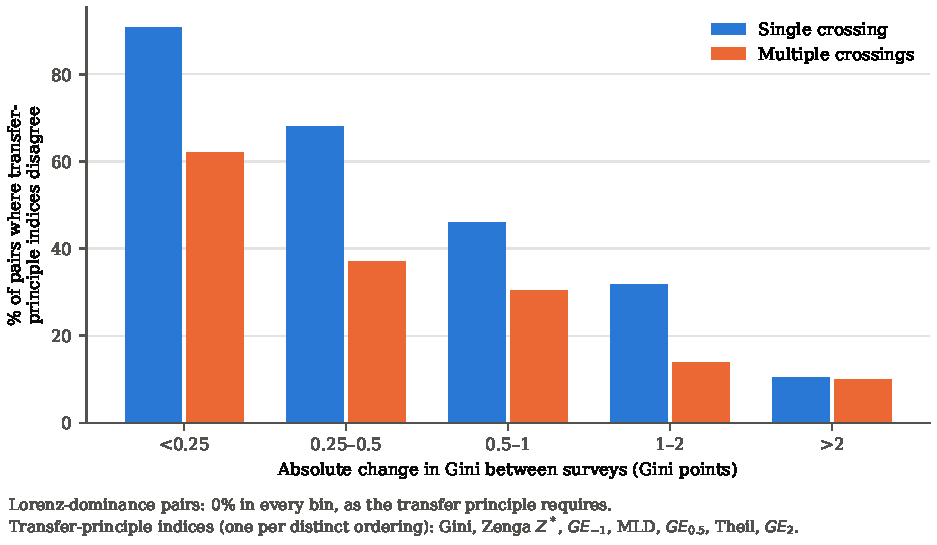
\includegraphics[width=0.85\textwidth]{../figures/pip_by_size.pdf}
\caption{Disagreement among transfer-principle indices, by size of change}
\label{fig:pip_size}
\begin{minipage}{0.85\textwidth}
\footnotesize
Notes: Share of consecutive comparable PIP survey pairs in which the seven transfer-principle indices do not all move in the same direction, by Lorenz relationship and by the absolute change in the Gini.
Under Lorenz dominance the share is zero in every bin, as Theorem~\ref{thm:dss} requires.
\end{minipage}
\end{figure}

Which indices disagree is predictable from their sensitivities (Figure~\ref{fig:pip_heat}).
Indices with similar weighting rarely conflict: the Gini and the MLD move in opposite directions in \PipDisGiniMld{} of pairs, and the Gini and $Z^*$ in \PipDisGiniZenga{}.
Indices that weight opposite ends of the distribution conflict often: $GE_2$, which is sensitive to the top, and the Atkinson index with $\varepsilon = 2$, which is sensitive to the bottom, disagree in \PipDisGeTwoAtkTwo{} of pairs.

\begin{figure}[H]
\centering
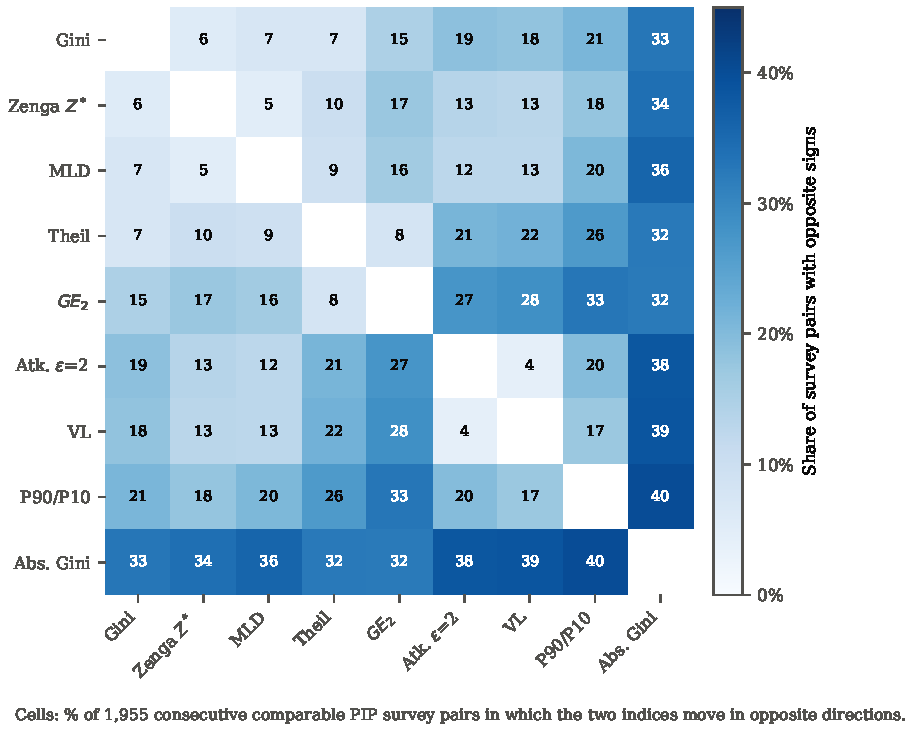
\includegraphics[width=0.72\textwidth]{../figures/pip_disagreement.pdf}
\caption{Pairwise disagreement on the direction of change}
\label{fig:pip_heat}
\begin{minipage}{0.72\textwidth}
\footnotesize
Notes: Each cell is the percentage of the \PipPairs{} survey pairs in which the two indices change in opposite directions.
\end{minipage}
\end{figure}

\subsection{Relative Versus Absolute}

The Gini and the absolute Gini move in opposite directions in \PipDisGiniAbs{} of pairs, a rate matched among relative indices only by pairs that weight opposite tails, such as $GE_2$ and the 90/10 ratio (\PipDisGeTwoPNinety{}).
The conflict has a simple arithmetic source.
Since $\Delta \ln(\mu G) = \Delta \ln \mu + \Delta \ln G$, the absolute Gini rises whenever growth in the mean exceeds the proportional fall in the Gini.
In the PIP pairs the median absolute change in log mean income is \PipMedGrowth{} percent, against \PipMedDlnGini{} percent for the log Gini, and growth is the larger of the two in \PipShareGrowthExceeds{} of pairs.
Hence, in \PipOppGiniDownAbsUp{} of the conflicts relative inequality falls while absolute inequality rises.
Among the \PipNGrowth{} pairs in which mean income rose, the Gini fell in \PipGiniFellGrowth{}, and in \PipAbsUpGivenGiniDownGrowth{} of those the absolute Gini rose.
Over the \PipLongN{} comparable spells that span at least ten years, the Gini fell with rising mean income in \PipLongNGiniDownGrowth{} spells, and the absolute Gini rose in \PipLongAbsUpGivenGiniDown{} of them.
The choice of absolute index matters little: the Kolm index moves in the same direction as the absolute Gini in \PipKolmAgree{} of pairs and the standard deviation in \PipSdAgree{}, although the Kolm index depends on the unit of $\kappa$, which has to be fixed across countries whose mean incomes differ by a factor of more than \PipIncomeRange{}.

The consequence is that Lorenz dominance, which settles the comparison for every relative index satisfying the transfer principle, does not settle the absolute one.
Among the \PipNMaterialDom{} pairs in which the Gini moves by at least one point and one Lorenz curve dominates, the seven relative indices agree by Theorem~\ref{thm:dss}, but the absolute Gini moves the other way in \PipRelAbsOppMaterialDom{}.
This reversal holds for both welfare concepts, though it is more common among income surveys (\PipRelAbsOppMaterialDomIncome{}) than consumption surveys (\PipRelAbsOppMaterialDomConsumption{}).
In the \PipNMaterialCross{} crossing pairs with changes of the same size, the relative and absolute Gini conflict in \PipRelAbsOppMaterialCross{}, about as often as the relative indices conflict among themselves (\PipTpDisMaterialCross{}).
Taking all \PipNMaterial{} large changes together, the relative and absolute Gini conflict in \PipRelAbsOppMaterial{} of pairs and the relative indices in \PipTpDisMaterial{}.
Figure~\ref{fig:pip_countries} shows four cases.
In China between \PipChinaYears{}, the Gini of consumption rose from \PipChinaGiniA{} to \PipChinaGiniB{}, while mean consumption grew by a factor of \PipChinaMeanRatio{} and the absolute Gini by a factor of \PipChinaAbsRatio{}.
In Brazil between \PipBrazilYears{}, the last decade of the spell in the figure, the Gini fell from \PipBrazilGiniA{} to \PipBrazilGiniB{}, yet the absolute Gini rose by a factor of \PipBrazilAbsRatio{} because mean income grew faster than relative inequality fell.
In the United States and the United Kingdom the Gini ends within about ten percent of its starting value while the absolute Gini rises by up to a factor of two in the United States.
The same disagreement drives the debate over global inequality \citep{Ravallion2004,Atkinson2010,NinoZarazua2017}; the PIP data quantify it for national trends in \PipCountries{} countries.

\begin{figure}[H]
\centering
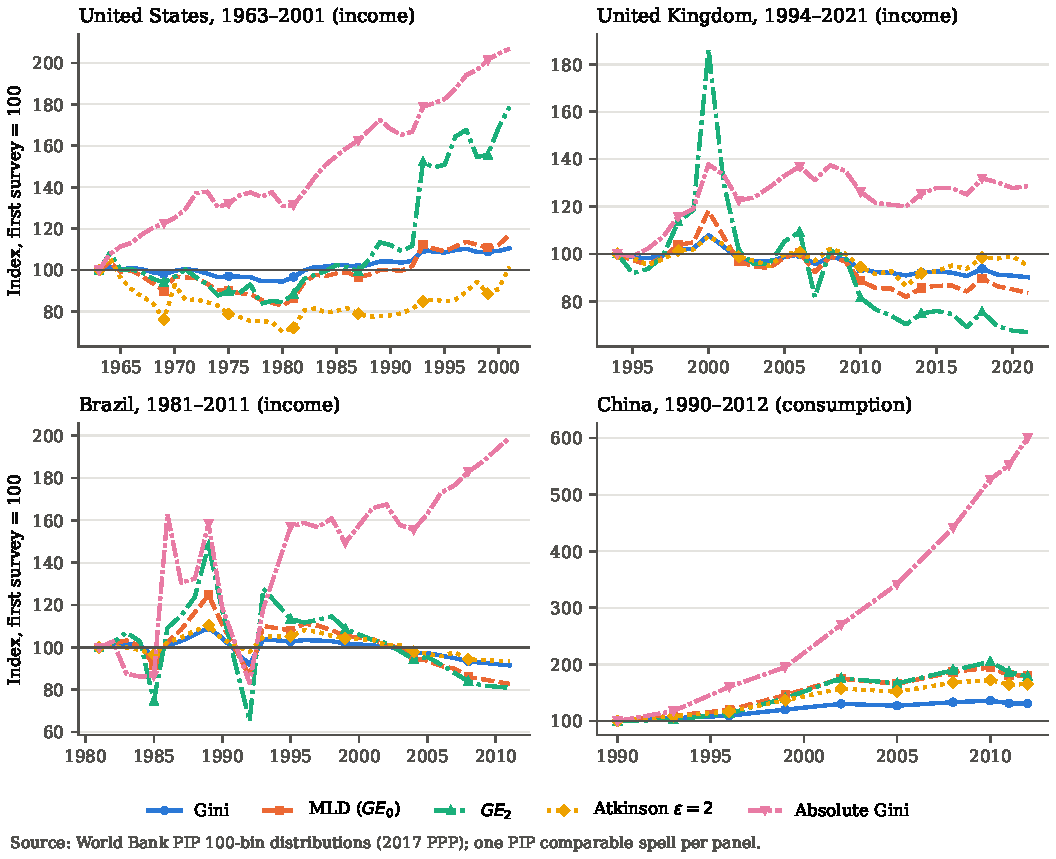
\includegraphics[width=\textwidth]{../figures/pip_countries.pdf}
\caption{Relative and absolute indices over time in four countries}
\label{fig:pip_countries}
\begin{minipage}{\textwidth}
\footnotesize
Notes: Each index is set to 100 in the first survey of one long comparable PIP spell per country. The absolute Gini is $\mu G$ in 2017 PPP dollars per day. China's national distributions are synthesised by the platform from urban and rural surveys.
\end{minipage}
\end{figure}

% ============================================================
% SECTION 8: PRACTICAL GUIDANCE
% ============================================================
\section{Practical Guidance for Applied Researchers}\label{sec:guidance}

The results of the previous sections reveal a landscape of tradeoffs.
No single index satisfies all desirable properties, and the choice of measure should be guided by the research question.
We offer the following practical recommendations.

\textbf{If decomposability matters, use the GE family.}
For any study that requires decomposing inequality into within-group and between-group components---for example, decomposing wage inequality by education, gender, or race---the Generalized Entropy family is the only scale-invariant option (Theorem~\ref{thm:shorrocks}).
Within the GE family, the choice of $\alpha$ should reflect the researcher's judgment about which part of the distribution matters most:
\begin{itemize}
    \item $\alpha = 0$ (MLD): more sensitive to changes at the bottom than the Theil ($\alpha < 0$ is more so). Suitable for poverty-focused analyses.
    \item $\alpha = 1$ (Theil): balanced sensitivity; weights by income shares in decomposition. Suitable for general-purpose analysis.
    \item $\alpha = 2$ (half-squared CV): more sensitive to changes at the top ($\alpha > 2$ is more so). Suitable for analyses focused on top-income dynamics.
\end{itemize}

\textbf{If welfare-theoretic foundations matter, use the Atkinson index.}
The Atkinson index has a direct welfare interpretation through the equally distributed equivalent income.
It satisfies all properties except translation invariance and additive decomposability, and it satisfies subgroup consistency, which is often sufficient for practical purposes.
The parameter $\varepsilon$ has a clear interpretation as inequality aversion, making results transparent and facilitating sensitivity analysis.

\textbf{If simplicity and communication matter, the Gini is defensible---with caveats.}
The Gini coefficient is intuitive, bounded between 0 and 1, and has a geometric interpretation via the Lorenz curve.
It satisfies the transfer principle and Lorenz consistency.
However, researchers should be aware of its limitations: it cannot be decomposed additively, it fails subgroup consistency, and its transfer sensitivity depends on ranks rather than income levels.
It is a reasonable summary statistic but a poor tool for decomposition.

\textbf{Prefer the MLD to the variance of logarithms.}
The VL fails the Pigou-Dalton transfer principle, so it can rise after a transfer from rich to poor.
In the PIP data this failure never reversed a Lorenz ranking (Section~\ref{sec:empirics}), so VL trends for national distributions are unlikely to be misleading on this account; the risk is greater for distributions with long upper tails, where transfers among top incomes carry more weight.
The MLD ($GE_0$) is also built on logarithms, satisfies the transfer principle, and decomposes additively, so it is the natural replacement.

\textbf{Treat the Zenga index as a descriptive device.}
The Zenga curve $1 - M^{-}(p)/M^{+}(p)$ shows how inequality varies across quantiles, and $Z^*$ is population-invariant and satisfies the transfer principle.
But it fails diminishing transfer sensitivity and subgroup consistency (Propositions~\ref{prop:dts} and~\ref{prop:subgroup}), so it offers no axiomatic advantage over the Gini, and the split-point version $Z$ should be avoided when populations differ in size (Theorem~\ref{thm:zenga_impossibility}).

\textbf{Percentile ratios are complements, not substitutes.}
The 90/10 ratio and similar measures are useful descriptive statistics that are robust to outliers and easy to interpret.
However, they fail most axiomatic properties and should not be used as the sole measure of inequality.
They are best used alongside a full-distribution measure like a GE index or the Gini.

\textbf{Check the Lorenz curves first, and state the invariance axiom.}
If one Lorenz curve dominates the other, every relative index satisfying the transfer principle gives the same answer and the choice among them is immaterial.
If the curves cross, report indices that weight the bottom and the top differently, such as the Atkinson index with $\varepsilon = 2$ and $GE_2$, which disagree in \PipDisGeTwoAtkTwo{} of the PIP comparisons.
Above all, say whether the conclusion is about relative or absolute inequality: even when Lorenz dominance makes every transfer-principle relative index agree on a change of a Gini point or more, the absolute Gini disagrees in \PipRelAbsOppMaterialDom{} of the PIP comparisons (Section~\ref{sec:empirics}).

% ============================================================
% SECTION 9: CONCLUSION
% ============================================================
\section{Conclusion}\label{sec:conclusion}

We evaluated eight inequality indices against eleven properties and then asked how often the properties decide anything in survey data.

On the theory side, three points bear repeating.
The maximum number of properties one index can satisfy is ten, and a relative index ($GE_\alpha$, $\alpha < 2$) and an absolute index ($E_\kappa$) both reach it, so the relative--absolute choice cannot be settled by counting axioms (Theorem~\ref{thm:optimality}).
The GE family remains the only scale-invariant family that decomposes additively (Theorem~\ref{thm:shorrocks}).
The Zenga indices $Z$ and $Z^*$ satisfy the transfer principle (Zenga's own finite formula $Z_N$ does not), but none of the three satisfies diminishing transfer sensitivity or subgroup consistency, and its split-point form cannot be population-invariant (Theorem~\ref{thm:zenga_impossibility}).

On the empirical side, the transfer principle and the Lorenz ordering it implies settle the direction of change in relative inequality in only \PipShareDom{} of consecutive PIP survey pairs.
In the remaining pairs, relative indices that all satisfy the transfer principle often disagree, mostly about small changes; once the Gini moves by a point or more, they disagree in \PipTpDisMaterialCross{} of crossing pairs.
The variance of logarithms, whose failure of the transfer principle is a textbook warning, never contradicted a Lorenz ranking in our \PipNDom{} dominance pairs.
The relative--absolute split is different in kind: it persists where the transfer principle settles every relative comparison, with the absolute Gini moving against a Lorenz-dominance ranking in \PipRelAbsOppMaterialDom{} of the large changes in which one Lorenz curve dominates.
A researcher who reports whether inequality rose should therefore say which invariance axiom the answer rests on.


\section*{Statements and Declarations}

\noindent\textbf{Funding.} The authors received no funding for this work.

\noindent\textbf{Competing interests.} The authors have no relevant financial or non-financial interests to disclose.

\noindent\textbf{Author contributions.} Both authors contributed to the conception, analysis, and writing of the paper and approved the final manuscript.

\noindent\textbf{Data and code availability.} The percentile distributions and survey table are publicly available from the World Bank's Poverty and Inequality Platform (2017 PPP vintage) under a CC BY 4.0 licence.
The code, the raw and processed data, and scripts that reproduce every number, figure, and counterexample in the paper are available at \url{https://github.com/diomavro/inequality-indices}.

\singlespacing

\bibliographystyle{plainnat}
\bibliography{references}

\clearpage
\onehalfspacing
% ============================================================
% APPENDICES
% ============================================================
\appendix

\section{Proofs for Table~\ref{tab:summary}}\label{app:table}
\setcounter{theorem}{0}
\renewcommand{\thetheorem}{A.\arabic{theorem}}

% ---- 5.1 Anonymity ----
\subsection{Anonymity}

\begin{proposition}\label{prop:anon}
All eight indices satisfy anonymity.
\end{proposition}

\begin{proof}
Each index is defined as a symmetric function of the income vector: the variance, VL, and GE involve sums over individual incomes; the Gini involves a double sum of absolute differences; the Atkinson index involves a power-mean; percentile ratios depend on order statistics; and the Zenga index depends on order statistics through the lower and upper means.
In each case, permuting the elements of $\bfy$ does not change the value of the index.
\end{proof}

The universality of anonymity reflects its status as a minimal fairness requirement.
An inequality measure that treated otherwise identical individuals differently based on their label would be difficult to justify.

% ---- 5.1b Population Invariance ----
\subsection{Population Invariance}

\begin{proposition}\label{prop:pop}
The Var, CV, VL, Gini, $GE_\alpha$, $A_\varepsilon$, $R_{p/q}$, $Z_N$, and $Z^*$ satisfy population invariance.
The split-point Zenga average $Z$ does not.
\end{proposition}

\begin{proof}
The first seven indices depend only on summary statistics (means, ratios $y_i/\mu$, ranks, or order statistics as percentile fractions) that are unchanged by exact population replication.

\textbf{Zenga's $Z_N$ (satisfies).}
Replication multiplies every frequency $n_h$ and the population size by $k$, so the weights $n_h/n$ and the lower and upper means at each distinct value are unchanged.

\textbf{Empirical Zenga $Z^*$ (satisfies).}
Population replication does not change the empirical quantile function: $F^{-1}_{\bfy^{(k)}} = F^{-1}_{\bfy}$.
Hence $M^{-}(p)$, $M^{+}(p)$, and $Z^*$ are all invariant.

\textbf{Split-point average $Z$ (fails).}
$Z$ averages over $n - 1$ split points with equal weights.
Replicating the population from $n$ to $kn$ changes the number of split points from $n - 1$ to $kn - 1$, altering the set of lower-upper mean ratios.
\emph{Counterexample:} $Z(1, 3) = 0.667$ but $Z(1, 1, 3, 3) = 0.561$.
No non-trivial equal-weight average of a continuous function of the split-point ratios can satisfy population invariance (Theorem~\ref{thm:zenga_impossibility}).
\end{proof}

% ---- 5.2 Scale Invariance ----
\subsection{Scale Invariance}

\begin{proposition}\label{prop:scale}
The CV, VL, Gini, $GE_\alpha$ (all $\alpha$), $A_\varepsilon$ (all $\varepsilon > 0$), $R_{p/q}$, and the three Zenga indices satisfy scale invariance.
The variance does not.
\end{proposition}

\begin{proof}
\textbf{Variance (fails).}
$\operatorname{Var}(\lambda\bfy) = \frac{1}{n}\sum_{i=1}^n (\lambda y_i - \lambda\mu)^2 = \lambda^2 \operatorname{Var}(\bfy)$.
For $\lambda \neq 1$, this differs from $\operatorname{Var}(\bfy)$.

\textbf{CV (satisfies).}
$\operatorname{CV}(\lambda\bfy) = \frac{\lambda\sqrt{\operatorname{Var}(\bfy)}}{\lambda\mu} = \operatorname{CV}(\bfy)$.

\textbf{VL (satisfies).}
$\ln(\lambda y_i) = \ln\lambda + \ln y_i$.
The mean of logs shifts by $\ln\lambda$, so each deviation $\ln(\lambda y_i) - \overline{\ln(\lambda y)}$ equals $\ln y_i - \overline{\ln y}$.
Hence $\operatorname{VL}(\lambda\bfy) = \operatorname{VL}(\bfy)$.

\textbf{Gini (satisfies).}
$G(\lambda\bfy) = \frac{1}{2n^2 \lambda\mu}\sum_{i,j}|\lambda y_i - \lambda y_j| = \frac{\lambda}{2n^2\lambda\mu}\sum_{i,j}|y_i - y_j| = G(\bfy)$.

\textbf{$GE_\alpha$ (satisfies).}
For $\alpha \neq 0, 1$: $GE_\alpha(\lambda\bfy) = \frac{1}{\alpha(\alpha-1)}\left[\frac{1}{n}\sum\left(\frac{\lambda y_i}{\lambda\mu}\right)^\alpha - 1\right] = GE_\alpha(\bfy)$.
The cases $\alpha = 0$ and $\alpha = 1$ follow similarly, since the ratios $y_i/\mu$ are unchanged.

\textbf{$A_\varepsilon$ (satisfies).}
The Atkinson index depends only on the ratios $y_i/\mu$, which are invariant to scaling.

\textbf{$R_{p/q}$ (satisfies).}
$R_{p/q}(\lambda\bfy) = \frac{\lambda y_{(\lceil pn \rceil)}}{\lambda y_{(\lceil qn \rceil)}} = R_{p/q}(\bfy)$.

\textbf{Zenga (satisfies).}
Each ratio $\bar{y}^{-}_i / \bar{y}^{+}_i$ involves means of subsets of incomes.
Scaling by $\lambda$ multiplies both numerator and denominator by $\lambda$, so each ratio is unchanged, and hence $Z(\lambda\bfy) = Z(\bfy)$.\qedhere
\end{proof}

The failure of the variance to satisfy scale invariance is its most serious practical limitation.
If inequality in 1950 and 2020 is compared using the variance, real income growth alone will increase measured inequality even if the distribution has not changed in any relative sense.

% ---- 5.3 Translation Invariance ----
\subsection{Translation Invariance}

\begin{proposition}\label{prop:trans}
The variance satisfies translation invariance.
The CV, VL, Gini, $GE_\alpha$, $A_\varepsilon$, $R_{p/q}$, and the Zenga indices do not.
\end{proposition}

\begin{proof}
\textbf{Variance (satisfies).}
$\operatorname{Var}(\bfy + c\bfone) = \frac{1}{n}\sum_{i=1}^n (y_i + c - \mu - c)^2 = \frac{1}{n}\sum_{i=1}^n (y_i - \mu)^2 = \operatorname{Var}(\bfy)$.

\textbf{Others (fail).}
For $\bfy = (1, 3)$, $n = 2$, $\mu = 2$:
$G = \frac{1}{2n^2\mu}\sum_{i,j}|y_i - y_j| = \frac{|1-1| + |1-3| + |3-1| + |3-3|}{2 \cdot 4 \cdot 2} = \frac{4}{16} = 0.25$.

Now add $c = 10$: $\bfy' = (11, 13)$, $\mu' = 12$.
$G' = \frac{4}{2 \cdot 4 \cdot 12} = \frac{4}{96} \approx 0.042$.
Since $G' \neq G$, the Gini is not translation-invariant.
For the other normalized, continuous, scale-invariant indices, Theorem~\ref{thm:impossibility} shows that some uniform shift must change the index.
The two indices on our list that fail normalization or continuity also fail translation invariance on this example: $R_{90/10}(1, 3) = 3$ but $R_{90/10}(11, 13) = 13/11$, and $Z_N(1, 3) = 1/3$ but $Z_N(11, 13) = 1/13$.
\end{proof}

The variance is the only translation-invariant index in Table~\ref{tab:summary}; other translation-invariant indices, such as the absolute Gini $\mu G$ and the Kolm index, appear in Sections~\ref{sec:optimality} and~\ref{sec:empirics}.

% ---- 5.4 Transfer Principle ----
\subsection{The Pigou-Dalton Transfer Principle}

\begin{proposition}\label{prop:transfer}
The Var, CV, Gini, $GE_\alpha$ (all $\alpha$), $A_\varepsilon$ (all $\varepsilon > 0$), $Z$, and $Z^*$ satisfy the transfer principle.
The VL, $R_{p/q}$, and $Z_N$ do not.
\end{proposition}

\begin{proof}
\textbf{Variance (satisfies).}
Consider a progressive transfer of $\delta > 0$ from person $i$ to person $j$, where $y_i > y_j$ and $y_i - \delta \geq y_j + \delta$.
The mean is unchanged.
The change in variance is
\begin{align}
\Delta\operatorname{Var} &= \frac{1}{n}\left[(y_i - \delta - \mu)^2 + (y_j + \delta - \mu)^2 - (y_i - \mu)^2 - (y_j - \mu)^2\right] \nonumber\\
&= \frac{1}{n}\left[-2\delta(y_i - \mu) + \delta^2 + 2\delta(y_j - \mu) + \delta^2\right] \nonumber\\
&= \frac{2\delta}{n}\left[\delta - (y_i - y_j)\right]. \label{eq:var_transfer}
\end{align}
Since $y_i - y_j > 0$ and $\delta \leq (y_i - y_j)/2$, we have $\delta - (y_i - y_j) < 0$, so $\Delta\operatorname{Var} < 0$.

\textbf{CV (satisfies).}
Since the mean is unchanged and the variance decreases (by the argument above), $\operatorname{CV} = \sqrt{\operatorname{Var}}/\mu$ decreases.

\textbf{Gini (satisfies).}
Using the rank-weighted representation~\eqref{eq:gini_rank}, a progressive transfer that does not change ranks transfers income weight from a higher-ranked position to a lower-ranked position.
Formally, if the donor has rank $r_h$ and the recipient has rank $r_l < r_h$ (in ascending order), the change in the Gini is
\begin{equation}\label{eq:gini_transfer}
\Delta G = -\frac{2\delta(r_h - r_l)}{n^2\mu} < 0.
\end{equation}
This is negative since $r_h > r_l$, $\delta > 0$, and $\mu > 0$.
A transfer that changes the ranks of third parties can be split into a finite sequence of smaller transfers between the same two people, each of which preserves ranks, so the Gini falls in that case too.

\textbf{$GE_\alpha$ (satisfies, all $\alpha$).}
We prove this using the convexity/concavity of the generating function.

\emph{Case $\alpha > 1$ or $\alpha < 0$:} The function $g(y) = y^\alpha$ is strictly convex.
For any strictly convex function $g$ and a progressive transfer from $y_i$ to $y_j$ (with $y_i > y_j$, transfer amount $\delta$, $y_i - \delta \geq y_j + \delta$):
\begin{equation}
g(y_i - \delta) + g(y_j + \delta) < g(y_i) + g(y_j),
\end{equation}
which follows because the function's slope is steeper at $y_i$ than at $y_j$, so the loss at the top exceeds the gain at the bottom.
Since $GE_\alpha = \frac{1}{\alpha(\alpha-1)}\left[\frac{1}{n\mu^\alpha}\sum y_i^\alpha - 1\right]$ and $\frac{1}{\alpha(\alpha-1)} > 0$ for $\alpha > 1$ or $\alpha < 0$, the index decreases.

\emph{Case $0 < \alpha < 1$:} The function $g(y) = y^\alpha$ is strictly concave, so $\sum y_i^\alpha$ increases under a progressive transfer.
But $\frac{1}{\alpha(\alpha-1)} < 0$, so the product decreases.

\emph{Case $\alpha = 1$ (Theil):} The function $g(y) = y\ln y$ is strictly convex (since $g''(y) = 1/y > 0$), so $\sum y_i \ln y_i$ decreases.
Since the Theil index equals $\frac{1}{n\mu}\sum y_i\ln y_i - \ln\mu$ and $\mu$ is unchanged, the Theil decreases.

\emph{Case $\alpha = 0$ (MLD):} The function $g(y) = \ln y$ is strictly concave, so $\sum \ln y_i$ increases under a progressive transfer.
Since $MLD = \ln\mu - \frac{1}{n}\sum\ln y_i$ and $\mu$ is unchanged, the MLD decreases.

\textbf{$A_\varepsilon$ (satisfies).}
Since $A_\varepsilon$ is a monotonically increasing function of $GE_{1-\varepsilon}$, and $GE_{1-\varepsilon}$ satisfies the transfer principle, so does $A_\varepsilon$.

\textbf{Zenga (satisfies).}
Consider a progressive transfer of $\delta$ from the individual at rank $r_h$ to the individual at rank $r_l < r_h$ (in the sorted order), with $\delta$ small enough that ranks are preserved.
We show each pointwise ratio $Z_i = 1 - \bar{y}^{-}_i/\bar{y}^{+}_i$ weakly decreases, with strict decrease for $r_l \leq i < r_h$.

\emph{Case $i < r_l$:} Both individuals are in the upper group (ranks $i+1, \ldots, n$).
The donor loses $\delta$ and the recipient gains $\delta$, leaving the upper-group sum unchanged.
The lower mean $\bar{y}^{-}_i$ involves only ranks $1, \ldots, i$, none of which changed.
Hence $Z_i$ is unchanged.

\emph{Case $r_l \leq i < r_h$:} The recipient (rank $r_l$) is in the lower group and the donor (rank $r_h$) is in the upper group.
The lower mean increases: $\bar{y}^{-\prime}_i = \bar{y}^{-}_i + \delta/i$.
The upper mean decreases: $\bar{y}^{+\prime}_i = \bar{y}^{+}_i - \delta/(n-i)$.
Both changes increase the ratio $\bar{y}^{-}_i/\bar{y}^{+}_i$, so $Z_i = 1 - \bar{y}^{-}_i/\bar{y}^{+}_i$ strictly decreases.

\emph{Case $i \geq r_h$:} Both individuals are in the lower group.
The sum of lower-group incomes is unchanged ($+\delta$ and $-\delta$ cancel), so $\bar{y}^{-}_i$ is unchanged.
The upper mean involves neither individual, so $\bar{y}^{+}_i$ is unchanged.
Hence $Z_i$ is unchanged.

Since $Z_i$ strictly decreases for every split point $i \in \{r_l, \ldots, r_h - 1\}$ (a non-empty set) and is unchanged elsewhere, the Zenga index $Z = \frac{1}{n-1}\sum Z_i$ strictly decreases.
For transfers large enough to change ranks, decompose into a finite sequence of rank-preserving transfers, each strictly reducing $Z$.
For $Z^*$, a progressive transfer weakly raises the Lorenz curve $L$ everywhere and strictly on an interval, so $M^{-}(p) = \mu L(p)/p$ weakly rises and $M^{+}(p) = \mu[1 - L(p)]/(1 - p)$ weakly falls at every $p$, strictly on a set of positive measure, and $Z^*$ strictly falls.
$Z_N$ fails: the transfer from $(1, 1.2, 3)$ to $(1.1, 1.1, 3)$ raises it from $0.386$ to $0.422$ (Section~\ref{sec:zenga}).

\textbf{VL (fails).}
\emph{Counterexample.}
Let $\bfy = (1, 2, 50, 100)$ and consider a progressive transfer of $\delta = 10$ from the person with income 100 to the person with income 50, yielding $\bfy' = (1, 2, 60, 90)$.
Note that $100 - 10 = 90 \geq 60 = 50 + 10$, so this is a valid progressive transfer.

Computing the variance of logarithms:
\begin{align*}
\overline{\ln y} &= \frac{0 + 0.693 + 3.912 + 4.605}{4} = 2.303,\\
\operatorname{VL}(\bfy) &= \frac{(0-2.303)^2 + (0.693-2.303)^2 + (3.912-2.303)^2 + (4.605-2.303)^2}{4} \\
&= \frac{5.302 + 2.590 + 2.590 + 5.302}{4} = 3.946.
\end{align*}
After the transfer:
\begin{align*}
\overline{\ln y'} &= \frac{0 + 0.693 + 4.094 + 4.500}{4} = 2.322,\\
\operatorname{VL}(\bfy') &= \frac{(0-2.322)^2 + (0.693-2.322)^2 + (4.094-2.322)^2 + (4.500-2.322)^2}{4} \\
&= \frac{5.391 + 2.653 + 3.142 + 4.744}{4} = 3.982.
\end{align*}
Since $3.982 > 3.946$, the progressive transfer \emph{increased} the variance of logarithms.

The logarithm is a concave function that ``compresses'' high incomes: the difference between $\ln(50)$ and $\ln(100)$ is only 0.693, while the difference between $\ln(1)$ and $\ln(2)$ is also 0.693, despite a much smaller absolute gap.
When we transfer income between two high-income individuals, the transfer barely registers in log space.
But the transfer changes the mean of logs, which shifts all the deviations, and this indirect effect can dominate, perversely increasing the variance of logarithms.

\textbf{$R_{p/q}$ (fails).}
Percentile ratios depend only on two order statistics.
Any progressive transfer not involving the $p$-th or $q$-th percentile leaves the ratio unchanged.
Moreover, a transfer between individuals both above the $p$-th percentile or both below the $q$-th percentile has no effect.
\end{proof}

% ---- 5.5 Diminishing Transfer Sensitivity ----
\subsection{Diminishing Transfer Sensitivity}

\begin{proposition}\label{prop:dts}
$GE_\alpha$ satisfies diminishing transfer sensitivity if and only if $\alpha < 2$.
The Atkinson index $A_\varepsilon$ satisfies it for all $\varepsilon > 0$.
The variance, CV, Gini, and the three Zenga indices $Z$, $Z_N$, and $Z^*$ do not satisfy it.
\end{proposition}

\begin{proof}
\textbf{$GE_\alpha$.}
For every $\alpha$, $GE_\alpha(\bfy) = \frac{1}{n}\sum_i \phi_\alpha(y_i) + c$, where $c$ and the strictly convex function $\phi_\alpha$ depend on $\mu$ only, and $\phi_\alpha''(s) = s^{\alpha - 2}/\mu^\alpha$ (for $\alpha = 0$, $\phi_0(s) = -\ln s$; for $\alpha = 1$, $\phi_1(s) = (s/\mu)\ln s$ up to terms linear in $s$).
A transfer of $\delta$ from $y + d$ to $y$ leaves $\mu$ unchanged and reduces $n\,GE_\alpha$ by
\begin{equation}\label{eq:ge_sensitivity}
\Delta_\alpha(y) = \phi_\alpha(y) + \phi_\alpha(y + d) - \phi_\alpha(y + \delta) - \phi_\alpha(y + d - \delta) = \int_0^\delta \!\! \int_{t}^{d - \delta + t} \phi_\alpha''(y + s)\, ds\, dt,
\end{equation}
which holds for any transfer size.
The region of integration does not depend on $y$, so $\Delta_\alpha(y)$ is strictly decreasing in $y$ when $\phi_\alpha''$ is strictly decreasing ($\alpha < 2$), constant when $\alpha = 2$, and strictly increasing when $\alpha > 2$.
Hence $GE_\alpha$ satisfies DTS if and only if $\alpha < 2$, for every transfer size $\delta \leq d/2$.

\textbf{Variance and CV (fail).}
From equation~\eqref{eq:var_transfer}, the change in variance from a transfer of $\delta$ with gap $d = y_i - y_j$ is $\frac{2\delta}{n}[\delta - d]$, which depends on $d$ and $\delta$ but \emph{not} on the income level $y_j$.
Since CV$^2 = 2 \cdot GE_2$ and $GE_2$ has $\alpha = 2$ (the level-neutral case), the CV also fails DTS.

\textbf{Gini (fails).}
From equation~\eqref{eq:gini_transfer}, $|\Delta G| = \frac{2\delta(r_h - r_l)}{n^2\mu}$, which depends on the \emph{rank gap} $r_h - r_l$, not on income levels.
Counterexample: consider $\bfy = (1, 2, 3, 98, 99, 100)$.
A transfer of $\delta = 0.5$ from income 2 to income 1 has rank gap 1.
A transfer of $\delta = 0.5$ from income 99 to income 98 also has rank gap 1.
Both reduce the Gini by the same amount, violating DTS.

\textbf{$A_\varepsilon$ (satisfies).}
Since $A_\varepsilon$ is a monotone increasing function of $GE_{1-\varepsilon}$ and $1 - \varepsilon < 1 < 2$ for all $\varepsilon > 0$, the Atkinson index inherits DTS from $GE_{1-\varepsilon}$.
To see why a monotone increasing transformation $A_\varepsilon = \phi(GE_{1-\varepsilon})$ preserves DTS: a progressive transfer that reduces $GE_{1-\varepsilon}$ by a larger amount at income level $y$ than at $y' > y$ also reduces $A_\varepsilon = \phi(GE_{1-\varepsilon})$ by a larger amount at $y$ (since $\phi$ is increasing, larger reductions in the argument produce larger reductions in $\phi$).
Hence the relative ranking of transfer effects on $GE_{1-\varepsilon}$ is preserved under $\phi$, and DTS carries over to $A_\varepsilon$.

\textbf{Zenga (fails).}
Take $\bfy = (3, 6, 7, 7, 8)$ and two transfers of $\delta = 1/2$ across a gap of $d = 1$: the low transfer from $7$ to $6$ and the high transfer from $8$ to $7$.
DTS requires the low transfer to reduce inequality by more.
It reduces $Z$, $Z_N$, and $Z^*$ by $0.0123$, $0.0180$, and $0.0102$, whereas the high transfer reduces them by $0.0161$, $0.0547$, and $0.0171$.
For comparison, the MLD falls by $0.0012$ after the low transfer and by $0.0009$ after the high one, as DTS requires.
A transfer between adjacent ranks $r$ and $r+1$ changes only the split-point term at $r$; to first order the reduction in $Z$ is proportional to $[1/r + (1 - Z_r)/(n - r)]/\bar{y}^{+}_r$, with $Z_r = 1 - \bar{y}^{-}_r/\bar{y}^{+}_r$.
The second term grows as $r$ approaches $n$, so transfers near the top of the distribution can outweigh transfers near the bottom.
In simulations with log-normal incomes the high transfer still has the larger effect in about $2\%$ of random comparisons at $n = 100$ (companion code), so the failure does not disappear in large populations.
\end{proof}

The economic implications of this result are significant.
An index without diminishing transfer sensitivity treats a \$100 transfer between millionaires as equally inequality-reducing as a \$100 transfer between minimum-wage workers.
For researchers studying poverty-related inequality or evaluating progressive tax policies, choosing an index with DTS (such as Theil, MLD, or Atkinson) is essential.

% ---- 5.6 Additive Decomposability ----
\subsection{Additive Decomposability}

\begin{proposition}\label{prop:decomp}
The variance and $GE_\alpha$ (all $\alpha$) satisfy additive decomposability.
The CV, VL, Gini, $A_\varepsilon$, $R_{p/q}$, and the Zenga indices do not.
\end{proposition}

\begin{proof}
\textbf{Variance (satisfies).}
The standard ANOVA decomposition gives
\begin{equation}\label{eq:var_decomp}
\operatorname{Var}(\bfy) = \sum_{k=1}^K \frac{n_k}{n}\operatorname{Var}(\bfy_k) + \sum_{k=1}^K \frac{n_k}{n}(\mu_k - \mu)^2,
\end{equation}
where the first term is the population-weighted average of within-group variances and the second term is the variance of group means---which equals $\operatorname{Var}(\mu_1\bfone_{n_1}, \ldots, \mu_K\bfone_{n_K})$.
This fits the form of equation~\eqref{eq:decomp} with weights $w_k = n_k/n$.

\textbf{$GE_\alpha$ (satisfies).}
For all $\alpha$,
\begin{equation}\label{eq:ge_decomp}
GE_\alpha(\bfy) = \sum_{k=1}^K \frac{n_k}{n}\left(\frac{\mu_k}{\mu}\right)^\alpha GE_\alpha(\bfy_k) + GE_\alpha(\mu_1\bfone_{n_1}, \ldots, \mu_K\bfone_{n_K}).
\end{equation}
The weights are $w_k = \frac{n_k}{n}\left(\frac{\mu_k}{\mu}\right)^\alpha$.
For $\alpha = 0$ (MLD), $w_k = n_k/n$ (population shares).
For $\alpha = 1$ (Theil), $w_k = \frac{n_k}{n}\frac{\mu_k}{\mu}$ (income shares).
For $\alpha = 2$, $w_k = \frac{n_k}{n}\left(\frac{\mu_k}{\mu}\right)^2$.

To verify, consider the case $\alpha = 0$ (MLD):
\begin{align}
MLD(\bfy) &= \frac{1}{n}\sum_{i=1}^n \ln\frac{\mu}{y_i} = \frac{1}{n}\sum_{k=1}^K \sum_{i \in k} \left(\ln\frac{\mu}{\mu_k} + \ln\frac{\mu_k}{y_i}\right) \nonumber\\
&= \sum_{k=1}^K \frac{n_k}{n}\ln\frac{\mu}{\mu_k} + \sum_{k=1}^K \frac{n_k}{n} \cdot \frac{1}{n_k}\sum_{i \in k}\ln\frac{\mu_k}{y_i} \nonumber\\
&= MLD(\mu_1\bfone_{n_1}, \ldots, \mu_K\bfone_{n_K}) + \sum_{k=1}^K \frac{n_k}{n} MLD(\bfy_k). \label{eq:mld_decomp}
\end{align}

\textbf{A test for failure.}
In~\eqref{eq:decomp} the weights and the between-group term depend only on subgroup sizes and means.
So if two versions of one subgroup have the same size, mean, and index value, and the other subgroups are unchanged, an additively decomposable index must give the same total.
Exhibiting two such versions with different totals shows that no choice of weights works.

\textbf{Gini (fails).}
With $A = (3, 9)$, the subgroups $B = (2, 4, 6)$ and $B' = (2.6, 2.8, 6.6)$ both have mean $4$ and Gini $2/9$, but $G(A, B) = 0.283$ and $G(A, B') = 0.277$.
The Gini does decompose exactly when subgroups do not overlap in income; the failure comes from the overlap term, which depends on how the subgroup distributions interleave \citep{Bhattacharya1967}.

\textbf{$R_{p/q}$ (fails).}
For the 90/10 ratio, $A = (4, 14)$ with $B = (3, 5, 18)$ or $B' = (2, 12, 12)$: both versions of $B$ have mean $26/3$ and ratio $6$, but the ratio for the whole population is $6$ in the first case and $7$ in the second.

\textbf{Zenga (fails).}
The same construction works for $Z$, $Z_N$, and $Z^*$: with $A = (3, 9)$ and $B = (2, 4, 6)$, a second version of $B$ with the same mean and the same index value, of the form $(x, x + 0.2, 11.8 - 2x)$, changes the total index in each case (companion code).

\textbf{VL and $A_\varepsilon$ (fail).}
Each is scale-invariant and satisfies the other conditions of Theorem~\ref{thm:shorrocks}, including differentiability, but neither is a positive multiple of a GE index ($A_\varepsilon$ is a nonlinear transformation of $GE_{1-\varepsilon}$, and the VL is not a function of any single GE index), so by that theorem neither is additively decomposable.

\textbf{CV (fails).}
The CV is not differentiable at perfect equality, so we argue directly.
Take two subgroups with fixed sizes and means and vary the CV $c_1$ of the first.
Since $\operatorname{CV}^2 = 2\,GE_2$ is additively decomposable, the total CV equals $\sqrt{a c_1^2 + b}$ for constants $a > 0$ and $b > 0$ that do not depend on $c_1$.
Additive decomposability of the CV would require the total to be affine in $c_1$, but $\sqrt{a c_1^2 + b}$ is strictly convex in $c_1$ whenever $b > 0$, for instance whenever the subgroup means differ.
\end{proof}

A researcher studying the evolution of income inequality over time wants to know whether changes are driven by widening gaps between demographic groups (between-group) or by increasing dispersion within groups (within-group).
Only additively decomposable measures provide a clean answer.

% ---- 5.7 Subgroup Consistency ----
\subsection{Subgroup Consistency}

\begin{proposition}\label{prop:subgroup}
The Var, CV, $GE_\alpha$ (all $\alpha$), and $A_\varepsilon$ (all $\varepsilon > 0$) satisfy subgroup consistency.
The Gini, VL, $R_{p/q}$, and the three Zenga indices do not.
\end{proposition}

\begin{proof}
\textbf{Var and $GE_\alpha$ (satisfy).}
These indices are additively decomposable.
In the decomposition~\eqref{eq:decomp}, if the distribution in subgroup $k$ changes to $\bfy'_k$ with the same mean $\mu_k$ and $I(\bfy'_k) > I(\bfy_k)$, the between-group component is unchanged (since all group means and sizes are unchanged), and the within-group component increases (since $w_k > 0$ and the $k$-th term increases).
Hence total inequality increases.

\textbf{CV (satisfies).}
$\operatorname{CV}^2 = 2 \cdot GE_2$ is additively decomposable and satisfies subgroup consistency.
Since the CV is a monotone increasing function of $\operatorname{CV}^2$, it also satisfies subgroup consistency.

\textbf{$A_\varepsilon$ (satisfies).}
$A_\varepsilon$ is a monotone increasing function of $GE_{1-\varepsilon}$.
If within-group inequality increases (as measured by $A_\varepsilon$ in subgroup $k$), then $GE_{1-\varepsilon}$ in subgroup $k$ also increases (same monotone relationship).
By subgroup consistency of $GE_{1-\varepsilon}$, total $GE_{1-\varepsilon}$ increases, and hence total $A_\varepsilon$ increases.

\textbf{Zenga (fails).}
Let subgroup $A = (36, 18, 15)$ and subgroup $B = (28, 23, 2, 3)$, and replace $A$ by $A' = (33, 12, 24)$, which has the same size and mean ($23$).
Within the subgroup, $Z^*$ rises from $0.4356$ to $0.4589$.
For the whole population, $Z^*$ falls from $0.7253$ to $0.7122$.
The MLD rises in both the subgroup and the total, as subgroup consistency requires.
The same example works for the other two versions: $Z$ rises from $0.4931$ to $0.5167$ in the subgroup and falls from $0.7372$ to $0.7252$ in total, and $Z_N$ rises from $0.3287$ to $0.3445$ and falls from $0.6319$ to $0.6216$.
Random searches over small integer populations find violations in about $2\%$ of same-mean replacements for $Z$ and $Z^*$ (companion code).


\textbf{Gini (fails).}
The failure is consistent with the characterization of \citet{Shorrocks1988}, under which subgroup consistency together with the other standard axioms and scale invariance characterizes indices ordinally equivalent to a GE index, but a direct example is simpler.
A small example: replace subgroup $A = (19, 8, 8)$ by $A' = (13, 5, 17)$, which has the same size and mean, leaving $B = (15, 14, 13)$ unchanged.
The Gini of the subgroup rises from $0.210$ to $0.229$, but the Gini of the whole population falls from $0.167$ to $0.145$.

\textbf{VL (fails).}
Replace subgroup $A = (16, 16)$ by $A' = (18, 14)$, leaving $B = (2, 2)$ unchanged.
The VL of the subgroup rises from $0$ to $0.0158$, but the VL of the whole population falls from $1.0810$ to $1.0807$.

\textbf{$R_{p/q}$ (fails).}
Changes in the interior of a subgroup's distribution may not affect the overall percentile ratio, so increasing inequality within a subgroup can leave the overall $R_{p/q}$ unchanged.
\end{proof}

The failure of the Gini to satisfy subgroup consistency is one of its most significant limitations.
It means that the Gini can produce paradoxical results: inequality could increase in every region of a country, yet the national Gini could decrease due to changes in how regional distributions overlap.

% ---- 5.8 Lorenz Consistency ----
\subsection{Lorenz Consistency}

\begin{proposition}\label{prop:lorenz}
The Var, CV, Gini, $GE_\alpha$, $A_\varepsilon$, $Z$, and $Z^*$ satisfy Lorenz consistency.
The VL, $R_{p/q}$, and $Z_N$ do not.
\end{proposition}

\begin{proof}
By Theorem~\ref{thm:dss}, an anonymous index is Lorenz-consistent if and only if it satisfies the transfer principle.
The indices in the first list satisfy the transfer principle (Proposition~\ref{prop:transfer} and Section~\ref{sec:zenga}); the VL, $R_{p/q}$, and $Z_N$ do not.
\end{proof}

\begin{remark}
For indices that are also scale-invariant (CV, Gini, $GE_\alpha$, $A_\varepsilon$), Lorenz consistency extends to distributions with different means: if $\bfy$ Lorenz-dominates $\bfz$, then $I(\bfy) < I(\bfz)$, even when $\mu(\bfy) \neq \mu(\bfz)$.
The variance, lacking scale invariance, is Lorenz-consistent only for same-mean comparisons.
\end{remark}

\section{Proofs and Remarks for Section~\ref{sec:characterization}}\label{app:proofs}
\setcounter{theorem}{0}
\renewcommand{\thetheorem}{B.\arabic{theorem}}

\begin{proof}[Proof of Theorem~\ref{thm:impossibility}]
Suppose for contradiction that such an index $I$ exists.
Consider two-person distributions $\bfy = (1, x)$ for $x > 1$, and define $f(x) = I(1, x)$.
By normalization, $f(1) = 0$ and $f(x) > 0$ for $x > 1$.

We show that $f$ must be constant on $(1, \infty)$, contradicting normalization.

Fix any $x > 1$ and $x' > 1$.
Choose $c = \frac{x - x'}{x' - 1}$.
We verify that $c > -1$ (so the translation is valid) and that both components remain positive:
\begin{itemize}
    \item $1 + c = \frac{x - 1}{x' - 1} > 0$ since $x > 1$ and $x' > 1$.
    \item $x + c = \frac{x(x'-1) + x - x'}{x'-1} = \frac{xx' - x'}{x'-1} = \frac{x'(x-1)}{x'-1} > 0$.
\end{itemize}

Now apply translation invariance followed by scale invariance:
\begin{align}
f(x) = I(1, x) &= I(1 + c, x + c) && \text{(translation invariance)} \nonumber\\
&= I\!\left(1, \frac{x + c}{1 + c}\right) && \text{(scale invariance, dividing by $1+c > 0$).} \label{eq:impossible}
\end{align}

Computing the second argument:
\begin{equation}
\frac{x + c}{1 + c} = \frac{x + \frac{x - x'}{x'-1}}{\frac{x-1}{x'-1}} = \frac{\frac{x(x'-1) + x - x'}{x'-1}}{\frac{x-1}{x'-1}} = \frac{x'(x-1)}{x-1} = x'.
\end{equation}

Therefore $f(x) = f(x')$ for any $x, x' > 1$.
So $f$ is constant on $(1, \infty)$; call this constant $c_0$.

By normalization, $f(1) = 0$ and $c_0 > 0$ (since $f(x) > 0$ for $x > 1$).
But then $\lim_{x \to 1^+} f(x) = c_0 > 0 \neq f(1) = 0$, contradicting continuity.
\end{proof}

\begin{proof}[Proof of Theorem~\ref{thm:dss}]
\textbf{(i) $\Rightarrow$ (ii).}
Suppose $\bfy$ Lorenz-dominates $\bfz$ (with the same mean and population size).
By the Hardy--Littlewood--P\'olya theorem \citep{Hardy1934}, there exists a finite sequence of progressive transfers transforming $\bfz$ into $\bfy$.
Since $\bfy$ and $\bfz$ are not permutations of each other, the sequence contains at least one transfer; each transfer strictly reduces $I$ (by the transfer principle) and permutations leave it unchanged (by anonymity), so $I(\bfy) < I(\bfz)$.

\textbf{(ii) $\Rightarrow$ (i).}
If $\bfy$ is obtained from $\bfz$ by a progressive transfer, then $L_{\bfy}(p) \geq L_{\bfz}(p)$ for all $p$, with strict inequality at some $p$, because the bottom group that contains the recipient but not the donor gains $\delta$.
So $\bfy$ Lorenz-dominates $\bfz$, and Lorenz consistency gives $I(\bfy) < I(\bfz)$.
\end{proof}

\begin{proof}[Proof of Theorem~\ref{thm:zenga_impossibility}]
Consider $\bfy = (a, b)$ with $0 < a < b$ and $r = a/b \in (0, 1)$.
Then $I_f(a, b) = f(r)$.
The 2-fold replication $\bfy^{(2)} = (a, a, b, b)$ has three split points with ratios
\[
\phi(r) = \frac{3r}{r+2}, \qquad r, \qquad \psi(r) = \frac{2r+1}{3}.
\]
Population invariance gives $f(r) = \tfrac{1}{3}[f(\phi(r)) + f(r) + f(\psi(r))]$, i.e.,
\begin{equation}\label{eq:zenga_fe}
2f(r) = f(\phi(r)) + f(\psi(r)).
\end{equation}

For $r \in (0, 1)$, both $\phi(r)$ and $\psi(r)$ lie strictly between $r$ and $1$: they are contractions toward the fixed point $r = 1$.

Fix any $\delta \in (0, 1)$ and consider $f$ on $[\delta, 1]$.
Since $f$ is continuous on a compact set, $M := \max_{r \in [\delta, 1]} |f(r)|$ is attained at some $r^* \in [\delta, 1)$ (the case $r^* = 1$ gives $M = 0$, and we are done).
From~\eqref{eq:zenga_fe}, $f(r^*) = \tfrac{1}{2}[f(\phi(r^*)) + f(\psi(r^*))]$.
Since $\phi(r^*), \psi(r^*) \in (r^*, 1) \subseteq [\delta, 1]$ and $|f| \leq M$ on this interval, the average can equal $\pm M$ only if $f(\phi(r^*)) = f(\psi(r^*)) = f(r^*)$.
Iterating with $\psi$: $f(\psi^k(r^*)) = f(r^*)$ for all $k \geq 1$.
But $\psi^k(r^*) \to 1$ and $f(1) = 0$, so by continuity $f(r^*) = 0$, contradicting $|f(r^*)| = M > 0$.
Therefore $M = 0$ and $f \equiv 0$ on $[\delta, 1]$.

Since $\delta > 0$ was arbitrary, $f \equiv 0$ on $(0, 1]$.
Every ratio $\bar{y}^{-}_i/\bar{y}^{+}_i$ of sorted incomes lies in $(0, 1]$, so $I_f$ is identically zero; the values of $f$ above $1$ never enter the index.
\end{proof}

\begin{proof}[Proof of Theorem~\ref{thm:optimality}]
Part (i) is Theorem~\ref{thm:impossibility}.
Part (ii) collects Propositions~\ref{prop:anon}--\ref{prop:lorenz} for $GE_\alpha$: it is anonymous, normalized, continuous, population-invariant, and scale-invariant; it satisfies the transfer principle and hence Lorenz consistency (Theorem~\ref{thm:dss}); it satisfies DTS for $\alpha < 2$ (Proposition~\ref{prop:dts}); and it is additively decomposable and therefore subgroup-consistent.

Part (iii).
Anonymity, continuity, and population invariance are immediate from~\eqref{eq:expo}, and translation invariance holds because $\mu - y_i$ is unchanged when every income rises by $c$.
Normalization: by Jensen's inequality $\frac{1}{n}\sum_i e^{\kappa(\mu - y_i)} \geq e^{\kappa \cdot 0} = 1$, with equality if and only if all incomes are equal, since $x \mapsto e^{x}$ is strictly convex.
Transfer principle: $E_\kappa + 1$ is a sum of the strictly convex function $\phi(y) = e^{\kappa(\mu - y)}$, and a progressive transfer leaves $\mu$ unchanged, so the index strictly falls; Lorenz consistency follows by Theorem~\ref{thm:dss}.
Diminishing transfer sensitivity: a transfer of $\delta$ from $y + d$ to $y$ changes the index by
\[
\frac{1}{n}\left[\phi(y + \delta) + \phi(y + d - \delta) - \phi(y) - \phi(y + d)\right] = \frac{1}{n} e^{\kappa(\mu - y)}\left[e^{-\kappa\delta} + e^{-\kappa(d - \delta)} - 1 - e^{-\kappa d}\right].
\]
The bracket is negative and depends only on $\delta$ and $d$, so the reduction is proportional to $e^{-\kappa y}$ and strictly larger at lower $y$.
Additive decomposability: for subgroups $k$ with sizes $n_k$ and means $\mu_k$,
\[
E_\kappa(\bfy) + 1 = \frac{1}{n}\sum_k \sum_{i \in k} e^{\kappa(\mu - \mu_k)} e^{\kappa(\mu_k - y_i)} = \sum_k w_k \left[E_\kappa(\bfy_k) + 1\right], \qquad w_k = \frac{n_k}{n} e^{\kappa(\mu - \mu_k)},
\]
and $\sum_k w_k = E_\kappa(\mu_1\bfone_{n_1}, \ldots, \mu_K\bfone_{n_K}) + 1$, which gives~\eqref{eq:decomp} with positive weights depending only on subgroup sizes and means.
Subgroup consistency then follows from Proposition~\ref{prop:compatibility}(iii).
$E_\kappa$ is not scale-invariant: $E_\kappa(1, 3) \neq E_\kappa(2, 6)$ for every $\kappa > 0$.
\end{proof}

\begin{remark}[Dropping One Axiom]\label{rem:independence}
Four of the axioms in Theorem~\ref{thm:shorrocks} cannot be dropped without admitting indices outside the GE family.
\begin{enumerate}[label=(\roman*)]
    \item \emph{Normalization.}
    The index $I \equiv 0$ satisfies every other axiom but is zero for unequal distributions.

    \item \emph{Population Invariance.}
    $I_n(\bfy) = \frac{n-1}{n}\,GE_1(\bfy)$ satisfies the other axioms, with decomposition weights rescaled by $\frac{n-1}{n} \big/ \frac{n_k - 1}{n_k}$.
    But $I_2(1,3) = \frac{1}{2} \cdot 0.1308 = 0.0654$ while $I_4(1,1,3,3) = \frac{3}{4} \cdot 0.1308 = 0.0981$.

    \item \emph{Scale Invariance.}
    The variance satisfies the other axioms but $\operatorname{Var}(2,6) = 4 \neq 1 = \operatorname{Var}(1,3)$.

    \item \emph{Additive Decomposability.}
    The Atkinson index $A_\varepsilon$ satisfies the other axioms, including differentiability, and is not a multiple of any $GE_\alpha$, so by Theorem~\ref{thm:shorrocks} it is not additively decomposable.
\end{enumerate}
\end{remark}



\end{document}
